\chapter{Feed Forward Neural Networks}

The goal of the following chapters is to introduce different types of neural network. To do so, we first introduce some definitions needed. 

\section{Abstract Neurons}\label{abstractneurons}

\begin{definition}
    An \define{abstract neuron}, or simply \define{neuron}, is a tuple $(\vx,\vw,\phi,y)$ where
    \begin{itemize}
        \item $\vx^\intercal = (x_0,\cdots,x_n)$ is the \define{input vector}, usually $x_0=-1$
        \item $\vw^\intercal = (w_0,\cdots,w_n)$ is the \define{weight vector}, with $w_0 = b$, the bias.
        \item $\phi:\R\to\R$ is the \define{activation function} of the neuron.
        \item $y=\phi(\vx^\intercal\vw)$ is the output of the neuron
    \end{itemize}
\end{definition}

The goal of the neuron is to take a target $z$, and "learn" the target by tunning $\vw$ such that $\phi(\vx^\intercal\vw) \approx z$ 

\begin{definition}
    A \define{perceptron} is a neuron with input $\vx\in\{0,1\}^n$ and activation function
    \begin{equation*}
        \phi(x) = 
        \begin{cases}
            1 & \text{if } x \geq 0\\
            0 & \text{if } x < 0
        \end{cases}
    \end{equation*}
    $\phi$ is called the \define{Heaviside} step function
\end{definition}

\begin{example}
    Let $f^*:\{0,1\}^2\to\{0,1\}$ be $f^*(x,y)=x\textbf{ and }y$. \\
    A solution using the Heaviside step function uses $\vw^\intercal = (1.5,1,1)$. Then $\vx^\intercal\vw = -1.5+x+y$, or equivalently, we have the line $y=1.5-x$
    \begin{figure}
    \centering
    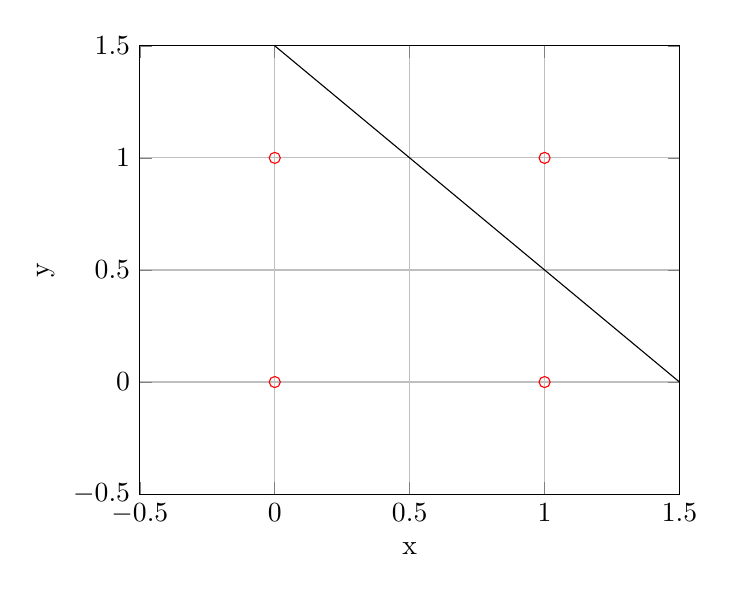
\begin{tikzpicture}
        \begin{axis}
        [
            xlabel={x}, 
            ylabel={y}, 
            grid, 
            xmin=-0.5, 
            xmax=1.5, 
            ymin=-0.5, 
            ymax=1.5, 
            tick align=inside
        ]
        \addplot[red, mark=o, only marks] coordinates {
            (0, 1)
            (0, 0)
            (1, 0)
            (1, 1)
        };
        \addplot[black] coordinates {(0, 1.5) (1.5, 0)};
        \end{axis}
    \end{tikzpicture}
    \caption{Outputs of \textbf{and} operator separated by $y=1.5-x$}
    \label{fig-heaviside-1}
\end{figure}
\end{example}

\begin{example}
    Let $f^*:\{0,1\}^2\to\{0,1\}$ be $f^*(x,y)=x\textbf{ or }y$. \\
    A solution using the Heaviside step function uses $\vw^\intercal = (0.5,1,1)$. Then $\vx^\intercal\vw = -0.5+x+y$, or equivalently, we have the line $y=0.5-x$
    \begin{figure}
    \centering
    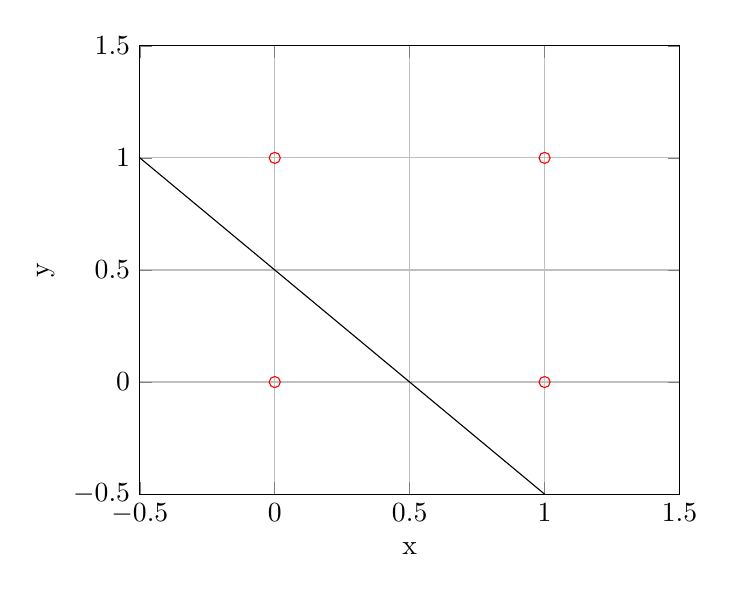
\begin{tikzpicture}
        \begin{axis}
        [
            xlabel={x}, 
            ylabel={y}, 
            grid, 
            xmin=-0.5, 
            xmax=1.5, 
            ymin=-0.5, 
            ymax=1.5, 
            tick align=inside
        ]
        \addplot[red, mark=o, only marks] coordinates {
            (0, 1)
            (0, 0)
            (1, 0)
            (1, 1)
        };
        \addplot[black] coordinates {(-0.5, 1) (1, -0.5)};
        \end{axis}
    \end{tikzpicture}
    \caption{Outputs of \textbf{or} operator separated by $y=0.5-x$}
    \label{fig-heaviside-2}
\end{figure}
\end{example}

The examples above illustrate that if the points cannot be divided by a line (or hyperplane in higher dimensions) then we cannot learn the function using a single neuron. We will fix this later by using multiple neurons.

\section{The Sigmoid Neuron}

To better predicting the value of binary variable y, we need to make sure there is a strong gradient. So we can use sigmoid output.

\begin{definition}
    A neuron with sigmoid activation $\sigma$ \\
    $\sigma$($w^T$$\vx$) is usually interpreted as the probability that target z = 1.
\end{definition}

Given a supervised dataset X,$\Vec{\vy}$, for $y_i$ $\in$ {0,1} and $\forall$ i sampled from $P_{data}$($\Vec{x}$,$\vy$), we can try to learn target y via prediction.\\

\centerline {y = 1 if $\sigma$($w^T$$\vx$) > 0.5} 
\centerline {y = 0 if $\sigma$($w^T$$\vx$) < 0.5}

Linear Neurons: Neurons with activation $\varphi$(x) = x

\begin{definition}
    ReLU(rectified linear unit)\\
    Activation function
    \begin{equation*}
        ReLU(X) = xH(x) = \begin{cases}
        1 & \quad x < 0, \\
        0 & \quad x > 0.
        \end{cases}
    \end{equation*}
\end{definition}

\begin{center}
    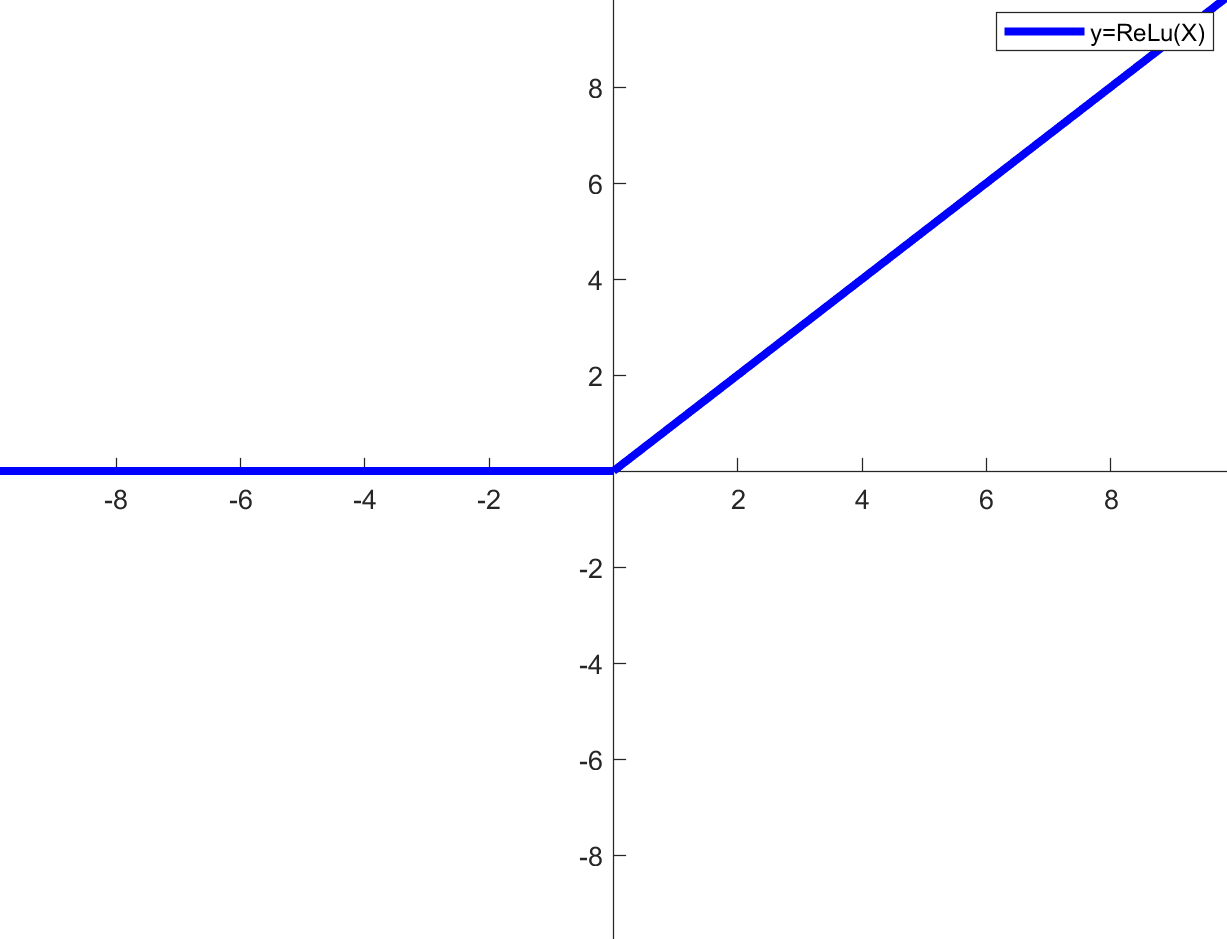
\includegraphics[width=2.1in]{images/Chapter 10/ReLU.png}
\end{center}


\begin{example}
    A Network of Neurons: \\
    \centerline{$f(\Vec{x})=\Vec{x_1}$ x or $\Vec{x_2}$, for $\Vec{x}$ $\in$ $\{0,1\}^2$}\\
    
    \centerline{
       dataset X = $
       \begin{bmatrix}
        0 & 1\\
        1 & 0\\
        0 & 1\\
        1 & 1
    \end{bmatrix}
    $,
    $\Vec{y}$ = $ 
    \begin{bmatrix}
        0\\
        1\\
        1\\
        0
        \end{bmatrix}$}
we can draw points in X in the folowing figure


\begin{center}
    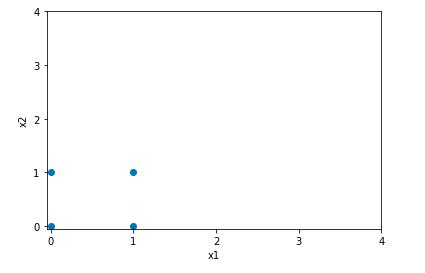
\includegraphics[width=3in]{images/Chapter 10/example1.png}
\end{center}




    Consider a modle f($\Vec{x}$,$\Vec{\theta}$) and cost function J($\theta$) = $\frac{1}{4}$ $\sum{(f^*(\Vec{x})-f(\Vec{x};\theta))}$

\begin{center}
    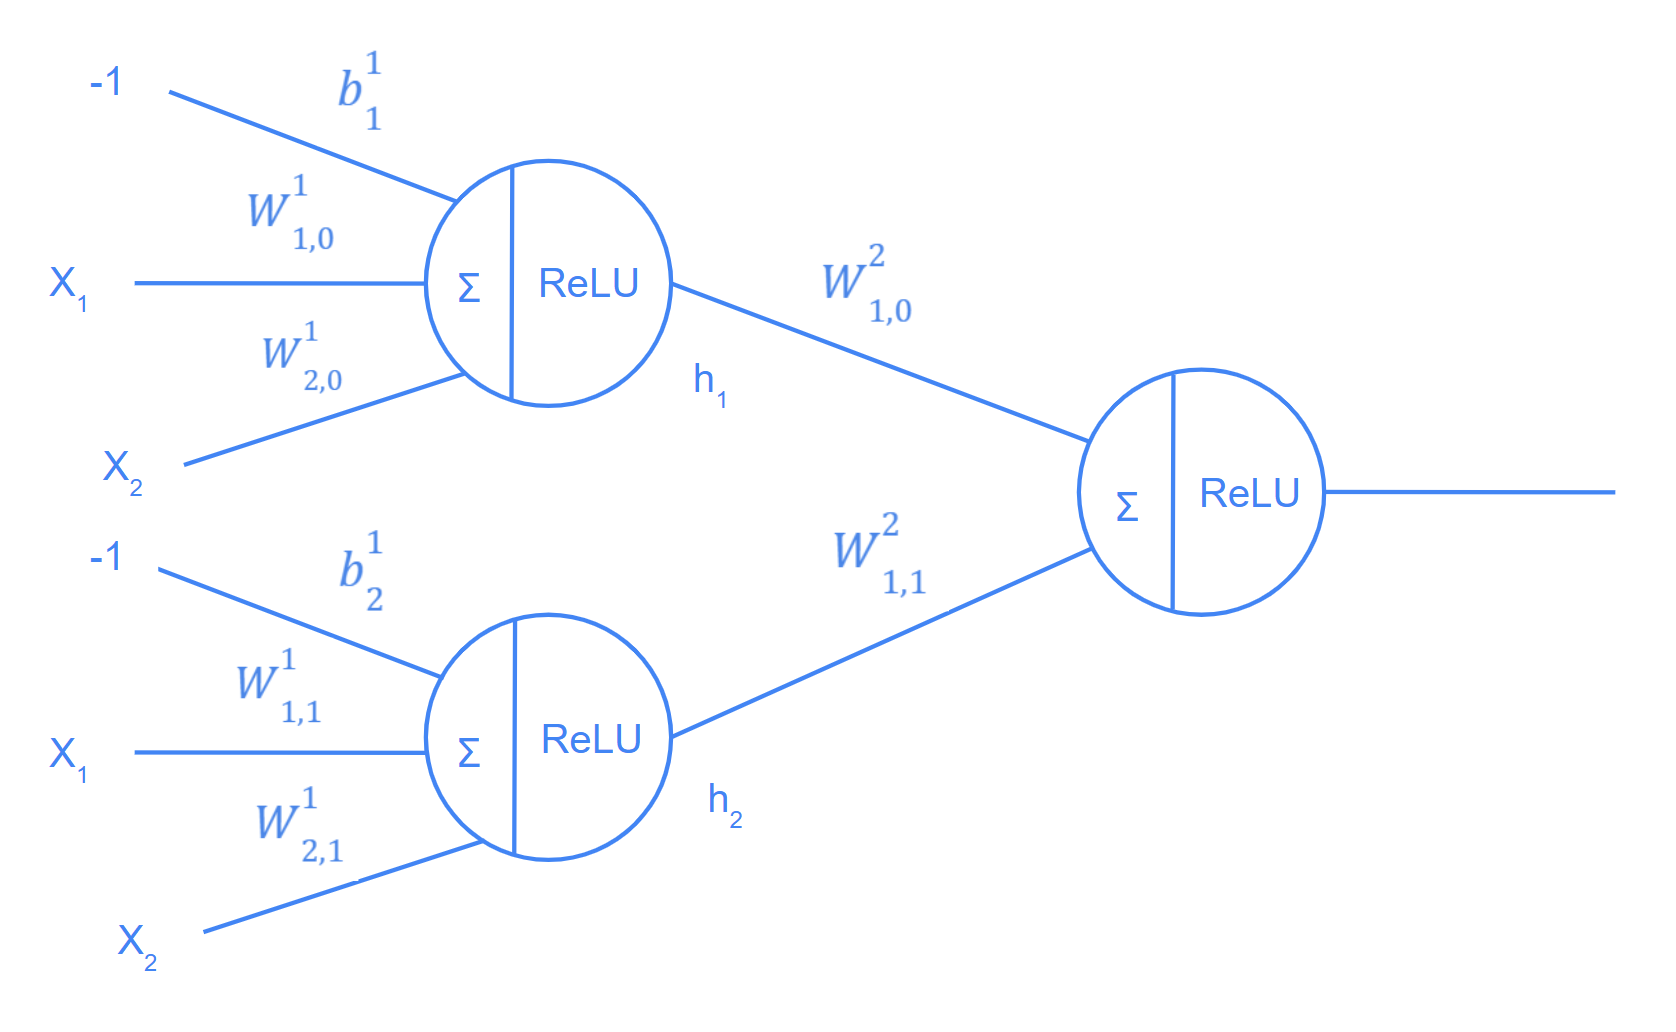
\includegraphics[width=3in]{images/Chapter 10/betterway.png}
\end{center}
    
    Idea: In $x_1$, $x_2$ - plane, the points are not separable by a line but maybe by transforing $x_1$, $x_2$ $\to$ $h_1$, $h_2$, the points can be separable by a line in the $h_1$, $h_2$ - plane.\\
    \centerline{
        $ \begin{pmatrix}
            h_{1}\\
            h_{2}
        \end{pmatrix} $ = ReLU($W^{(1)}\Vec{x}$ + $\vb^{(1)}$)
        }\\
    \centerline{
        Try $W^{(1)}$ = $ \begin{pmatrix}
            1 & 1\\
            1 & 1\\
        \end{pmatrix} $,
        $\Vec{\vb}^{(1)}$ = $ \begin{pmatrix}
            0\\
            -1
        \end{pmatrix} $
    }\\
    
    Apply to whole dataset.\\
    \begin{equation*}
         ReLU(XW^{(1)} + \Vec{1}\vb^{(1)}{}^T) = ReLU \left(
        \begin{pmatrix}
        0 & 0\\
        1 & 0\\
        0 & 1\\
        1 & 1
        \end{pmatrix} 
        \begin{pmatrix}
        1 & 1\\
        1 & 1
        \end{pmatrix} + 
        \begin{pmatrix}
        0 & -1\\
        0 & -1\\
        0 & -1\\
        0 & -1
        \end{pmatrix} \right)
    \end{equation*}
    \begin{equation*}  
        = ReLU \left(
        \begin{pmatrix}
        0 & 0\\
        1 & 1\\
        1 & 1\\
        2 & 2
        \end{pmatrix} 
        + \begin{pmatrix}
        0 & -1\\
        0 & -1\\
        0 & -1\\
        0 & -1
        \end{pmatrix} \right)
    \end{equation*}
    \begin{equation*}  
        = ReLU\begin{pmatrix}
        0 & -1\\
        1 & 0\\
        1 & 0\\
        2 & 1
        \end{pmatrix}\\
    \end{equation*}
    \begin{equation*}
        = \begin{pmatrix}
        0 & 0\\
        1 & 0\\
        1 & 0\\
        2 & 1
        \end{pmatrix}
    \end{equation*}


\begin{center}
    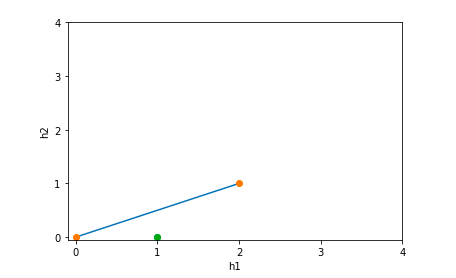
\includegraphics[width=4in]{images/Chapter 10/idea1.png}
\end{center}



So we can divide the point by y = $\frac{x}{2}$\\

Final output is
        $W^{(2)}$ $\begin{pmatrix}
        h_1\\
        h_2
        \end{pmatrix}$
        + $\vb^{(2)}$.
    Let $W^{(2)}$ = $\begin{pmatrix}
        1\\
        -2
        \end{pmatrix}$,
        $b^{(2)}$ = 0\\
        \begin{equation*}
            ReLU\left(
            \begin{pmatrix}
                0 & 0\\
                1 & 0\\
                1 & 0\\
                2 & 1
            \end{pmatrix}
            \begin{pmatrix}
                1\\
                -2
            \end{pmatrix}\right)
        \end{equation*}
        \begin{equation*}
            =ReLU
            \begin{pmatrix}
                0 \\
                1 \\
                1 \\
                0
            \end{pmatrix}
        \end{equation*}
        \begin{equation*}
            =\begin{pmatrix}
                0 \\
                1 \\
                1 \\
                0
            \end{pmatrix}
        \end{equation*}\\
        Better way to draw this:
    \begin{center}
        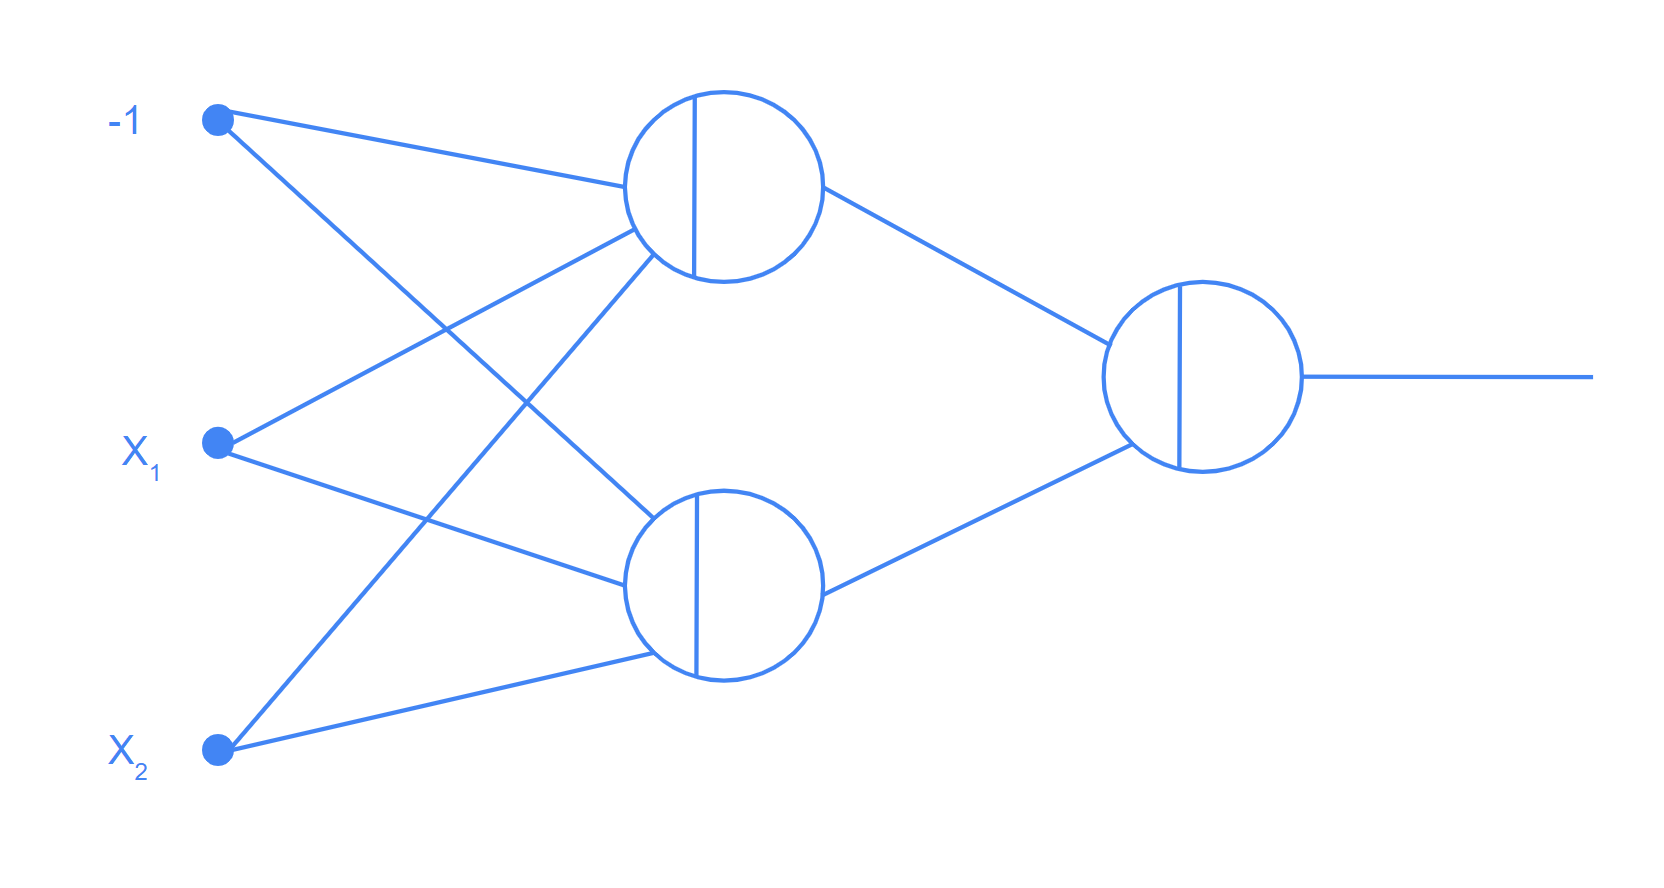
\includegraphics[width=3in]{images/Chapter 10/better.png}
    \end{center}
 \end{example}
 
 \begin{definition}
     A partially ordered set(poset) is a pair(P, $\leq$) where P is a set and $\leq$ is a relation on P s.t.\\
     1. x $\leq$ x, $\forall$ x $\in$ P\\
     2. if x $\leq$ y and y $\leq$ x then x = y $\forall$ x, y $\in$ P\\
     3.if x $leq$ y and y $\leq$ z then x $\leq$ z $\forall$ x, y, z $\in$ P
 \end{definition}

    Notation: Write x < y if x $\leq$ y and x $\neq$ y. Call (P, $\leq$) a total order if $\forall$ x, y $\in$ P x $\leq$ y or y $\leq$ x.\\
    
\begin{definition}
    A cover relation is a pair (x, y) s.t. x $\lneq$ y and $\nexists$ z with x < z < y.
\end{definition}

\begin{definition}
    The Hasse diagram of a finite poset (P, $\leq$) consists of a vertex for each x $\in$ P and a directed edge from x to y if and only if x $\in$ y draw from left to right. Write this as H(p).
\end{definition}

\begin{example}
    1.P = \{a, b, c, d\} a $\lneq$ b $\lneq$ c $\lneq$ d
    \begin{center}
        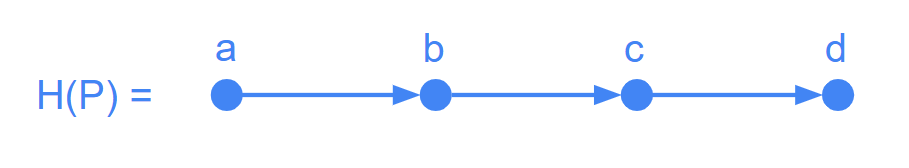
\includegraphics[width=2in]{images/Chapter 10/abcd.png}
    \end{center}
    2. P = \{S $\subseteq$ $\{1,2,3\}$ | S $\neq$ $\emptyset$ \} ordered by containment.
    \begin{center}
        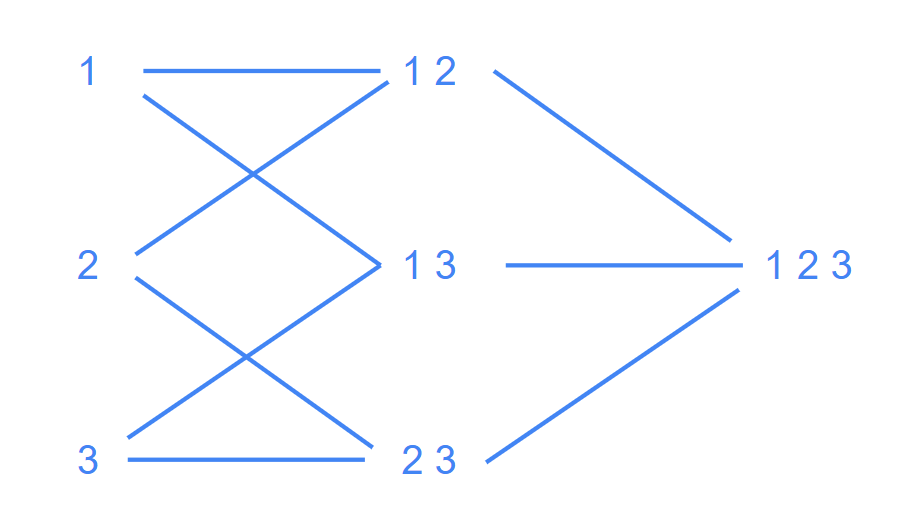
\includegraphics[width=2in]{images/Chapter 10/P123.png}
    \end{center}
\end{example}

\begin{definition}
    A poset is graded if $\exists$ P: P $\rightarrow$ $\mathbb{N}$ (rank function) such that\\
    1. x < y $\implies$ $\rho$(x) < $\rho$(y), $\forall$ x, y $\in$ P\\
    2. x $\leftarrow$ y $\implies$ $\rho$(x) + 1 = $\rho$(y), $\forall$ x, y $\in$ P
\end{definition}

\begin{example}
    \{S $\subseteq$ {1,2,3} | S $\neq$ $\emptyset$ \} is graded \\
    i.e. in a graded poset there is a notiton of "depth"
\end{example}

Following is an example of not graded
\begin{center}
        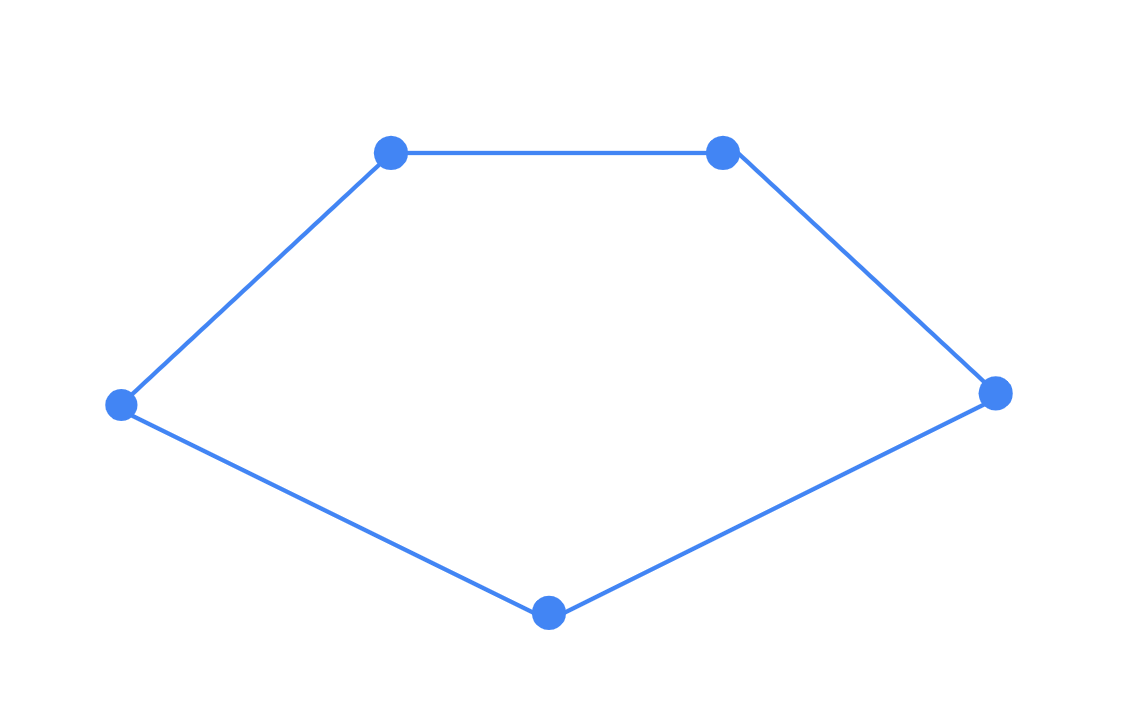
\includegraphics[width=2in]{images/Chapter 10/nonbigraded.png}
\end{center}


The rank decomposition of a graded poset (P, $\leq$, $\rho$) is
\begin{equation*}
    P = \oplus Pi, Pi = \{ x \in P | \rho(x) = i \}
\end{equation*}

\begin{center}
    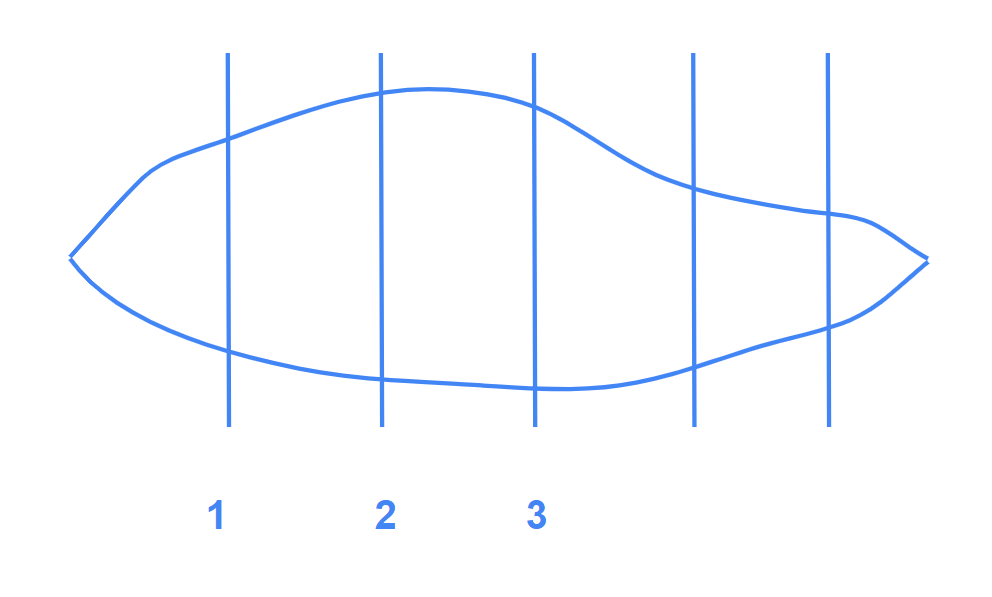
\includegraphics[width=2in]{images/Chapter 10/gradedp.png}
\end{center}

A linear extension of a poset (P, $\leq$) is a total ordering $\leq'$ on P s.t. x $\leq'$ y, for any x, y $\in$ P.\\
e.g\\.
\begin{center}
        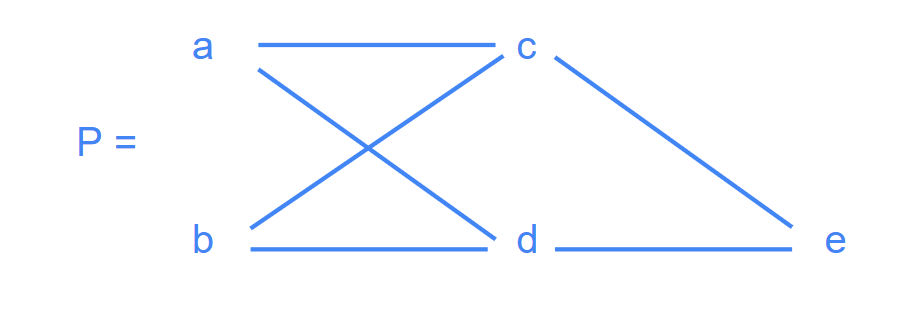
\includegraphics[width=2in]{images/Chapter 10/linear.png}
\end{center}
b < a < c < d < e\\

\begin{lemma}
    A linear extension of a graded poset is determined by a choice of total ordering of each of its ranks. So there are $\prod_{i \in \mathbb{N}}$ |$P_{i}$|\\
\end{lemma}

Convention Drawing a Hasse diagram determines a linear extension by ordering downwards along ranks: $a < b < c < d < e < f$.\\
    \begin{center}
        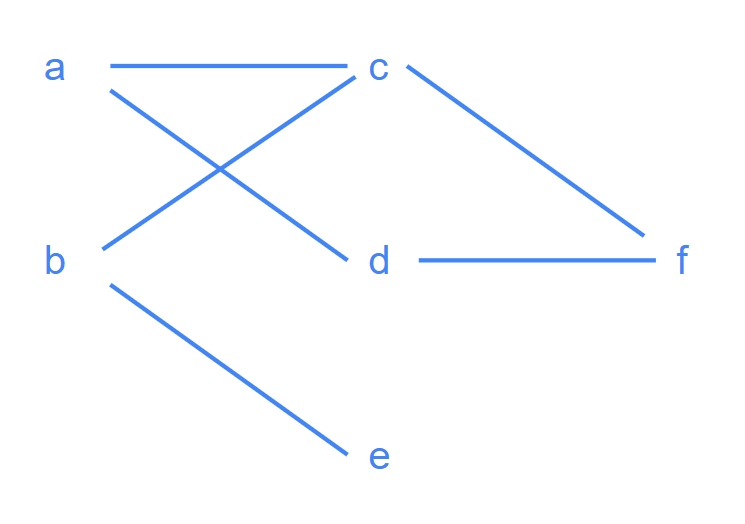
\includegraphics[width=2in]{images/Chapter 10/convention.png}
    \end{center}
So Hasse diagram contains all information.\\


\begin{definition}
    Let $N = (H,F,G)$ be a neural network with depth D and architecture $H$ = (P, $\leq$, $\rho$, $\leq'$).\\
    The feedforward of ${\vx} \in \mathbb{R}^{dim(V)_p^{D}}$ is:\\
        $N{\vx} = G_{D}F_{D-1}...G_{2}F_{1}G_{1}F_{0}{\vx} \in \mathbb{R}^{dim(V)_p^{D}}$
\end{definition}

\begin{example}
    Consider $N$ to be the following:\\
    \begin{center}
    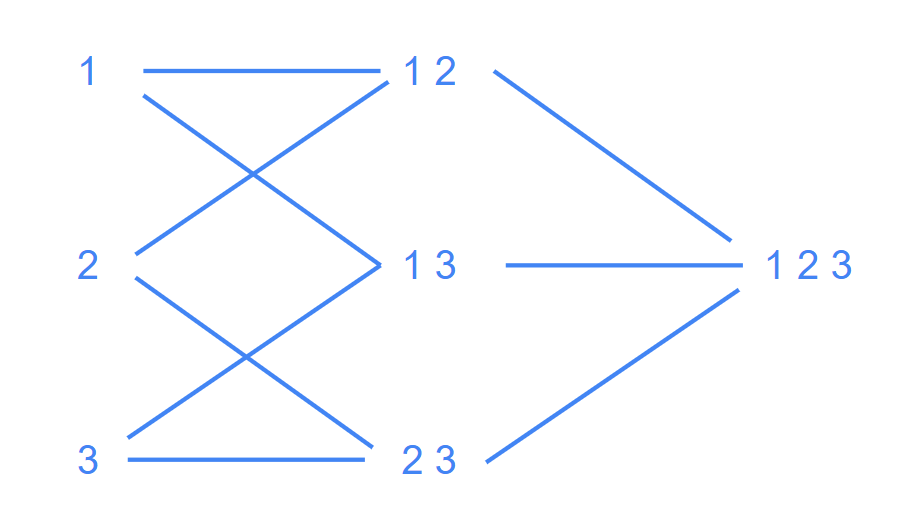
\includegraphics[width=2in]{images/Chapter 10/P123.png}
    \end{center}
    
     In this example, $${\vb}^{0} = \begin{pmatrix}1\\1\\1\\
        \end{pmatrix}$$ and ${\vb}^{1} = 0$
    We have $$N\begin{pmatrix}1\\1\\1\\
        \end{pmatrix} = G^{2}F^{1}G^{1}F^{0}\begin{pmatrix}1\\1\\1\\
        \end{pmatrix}$$
        So
        $$F^{0}{\vx} = \begin{pmatrix}1 & -1 & 0\\2 & 0 & 3\\0 & -2 & -3\\
        \end{pmatrix}{\vx}  + \begin{pmatrix}1\\1\\1\\
        \end{pmatrix}$$
        and
        $$F^{1}{\vx} = \begin{pmatrix}
        1 & -2 & 1
        \end{pmatrix}$$

    So now we get:
    
    $$N\begin{pmatrix}
    1\\1\\1\\ 
    \end{pmatrix} = 
    \sigma F^{1}ReLU F^{0} 
    \begin{pmatrix}1\\1\\1\\
    \end{pmatrix} = 
    \sigma F^{1}ReLU 
    \begin{pmatrix}1\\6\\-4\\
    \end{pmatrix} = 
    \sigma  F^{1} \begin{pmatrix}1\\6\\0\\
    \end{pmatrix} = 
    \sigma(-1\phi) = \frac{1}{1+e^{11}}$$
    
    which is approximately equal to 0.0001.
           
        
\end{example}

\begin{example}
Suppose that $N$ has some depth D and $G^{1},...,G^{D}$ are all linear activations ($G^{i}{\vx} = {\vx}$ $\forall i$). Then $N{\vx} = F^{D-1}F^{D-2}...F^{1}F^{0}{\vx}$.
    \begin{remark}
        The composition of affine maps is an affine map, so $\exists W, {\vb}$ such that $N{\vx} = W{\vx} + {\vb}$. So this Neural network can only fit affine functions, in other words, this is essentially linear regression.
    \end{remark}
\end{example}

\section{Neural Networks as Learning Algorithms}
Suppose there is a function $f^{*}:\mathbb{R}^{n} \mapsto \mathbb{R}^{k}$ (often k = 1) and we want to approximate or "model" $f^{*}$. Let $N$ be a neural network $N = (H,F,G)$ with depth D and $H = (P, \leq , \rho , \leq' )$ such that\\
 $\#P^{0} = n$ and $\#P^{D} = k$.\\
 \\
 Then we get $F^{i}{\vx} = W^{i}{\vx} + {\vb}^{i}$, where nonzero entries of $W^{i}$, and ${\vb}^{i}$ are treated as parameters.\\
 \\
 Let $W = (W^{0},...,W^{D-1})$ and $B = ({\vb}^{0},...,{\vb}^{D-1})$ and define $f_{model}({\vx};W,B) = N{\vx}$. (feedforward ${\vx}$).\\
 Now how do we find the appropriate values of W,B?\\
 Given a dataset $X \in \mathbb{R}^{mxn}$ and $Y \in \mathbb{R}^{mxk}$, we define a cost function:\\
\\
 $J(W,B) = \frac{1}{m} \sum_{i=1}^{m} L(f_{model}({\vx}^{i};W,B),{\vy}^{i})$.\\
and try to find values for W,B which minimize this cost function using some optimization algorithm.\\
\begin{note}
We will usually need to add a regularization term, which will be mentioned later in this chapter.\\
\\
A common choice for L is:\\
$L(f_{model}({\vx};W,B),{\vy}) = \norm{f_{model}({\vx};W,B) - {\vy}}_{2}^{2}$\\
\end{note}

\section{Neural Networks as a maximum likelihood estimator}
Lets assume X and Y are sampled from a distribution $p_{data}({\vx},{\vy})$ under I.I.D. assumptions.
Now let $p_{model}({\vy}|{\vx};\theta)$ be a model for $p_{data}({\vy}|{\vx})$, which has been parameterized by $\theta \in \mathbb{R}^{N}$ for some N.
Then $\theta_{ML} = \underset{\theta}{\mathrm{argmin}}(-\sum_{i=1}^{m}log(p_{model}({\vy}^{i}|{\vx}^{i};\theta))) $.

\begin{example}
Suppose we choose $P_{model}$ to be Gaussian:\\
$P_{model}({\vy}|{\vx};W,B) =$ N$({\vy};N{\vx},\sum)$ where N is the normal distribution and $N$ is the neural network.\\
\\
Then $P_{model}({\vy}|{\vx};W,B) =$ N$({\vy};N{\vx},\sum)$ = $\frac{1}{\sqrt{2\pi^{n}det\sum}}exp(-\frac{1}{2}({\vy}-N{\vx})\sum^{-1}({\vy}-N{\vx}))$ where\\ $N = (H,F,G)$,\\ $F_{\vx}^{i} = W^{i}{\vx} + {\vb}^{i}$,\\ $W = (W^{0},...,W^{D-1})$, and\\ $B = ({\vb}^{0},...,{\vb}^{D-1})$.\\
\\
Then finding $\theta_{ML} = (W,B)_{ML}$ is equivalent to minimizing our cost function of the form:\\
$J(W,B) = -\sum_{i=1}^{m}log(\frac{1}{\sqrt{2\pi^{n}det\sum}}exp(-\frac{1}{2}({\vy}^{i}-N{\vx}^{i})\sum^{-1}({\vy}^{i}-N{\vx}^{0})))$\\
= $\frac{1}{m}\sum-log(\frac{1}{constant}+\frac{1}{2}({\vy}^{i}-N{\vx}^{i})\sum^{-1}({\vy}^{i}-N{\vx}^{i})$, which $\frac{1}{constant}$ does not affect argmin, so we can ignore this value.\\
Then:\\
$J(W,B) = \frac{1}{m}\sum_{i=1}^{m}\frac{1}{2}({\vy}^{i}-N{\vx}^{i})\sum^{-1}({\vy}^{i}-N{\vx}^{i})$.\\
    \begin{note}
        We can usually take $\sum = id$ by first normalizing the dataset if needed.
    \end{note}
which then we get:\\
$J(W,B) = \frac{1}{m}\sum_{i=1}^{m}\norm{{\vy}^{i}-N{\vx}^{i}}^{2}_{2}$.\\
\\
In the end, we cycle back to our previous cost function.\\
    \begin{note}
        So we can either specify a cost or specify a model for $p_{data}$ and can usually go back and forth between those.
    \end{note}
\end{example}
                     
     

\section{Exercises}
\begin{enumerate}
    \item Given X,${\vy}$, using sigmoid, ReLU, then sigmoid function to rectified linear unit.
       \begin{equation*}  
        X = \begin{pmatrix}
        2 & 1 & 1\\
        0 & 1 & 0\\
        0 & -3 & 2\\
        2 & -2 & 2
        \end{pmatrix},
        \vb^{(1)} = \begin{pmatrix}
         1\\
         0\\
         0\\
         1
        \end{pmatrix},
        \vb^{(2)} = \begin{pmatrix}
         1\\
         1\\
         1\\
         1
        \end{pmatrix},
        \vw^{(1)} =  \begin{pmatrix}
         0.5 & 1 & 2\\
         1 & 2 & 0.5\\
         2 & 0.5 & 1
        \end{pmatrix}
        \end{equation*}
        \begin{equation*}
         w^{(2)} =  \begin{pmatrix}
         1 & 2 & 0.5\\
         1 & 2 & 0.5\\
         1 & 2 & 0.5
        \end{pmatrix}
         \vw^{(3)} =  \begin{pmatrix}
         1\\
         0.5\\
         2
        \end{pmatrix},
        \vb^{(3)} = \begin{pmatrix}
         0\\
         1\\
         1\\
         0
        \end{pmatrix}
        \end{equation*}
    \item Draw a linear extension of poset (P, $\leq$), a < b < c < d < e < f
    \item Explain why we use sigmoid activation function to predict value of binary variable y.
    \item Determine the weight matrices $W^{(0)}, W^{(1)}, W^{(3)}, W^{(4)}$ for the following neural network if all connection weights are worth 1.
    
    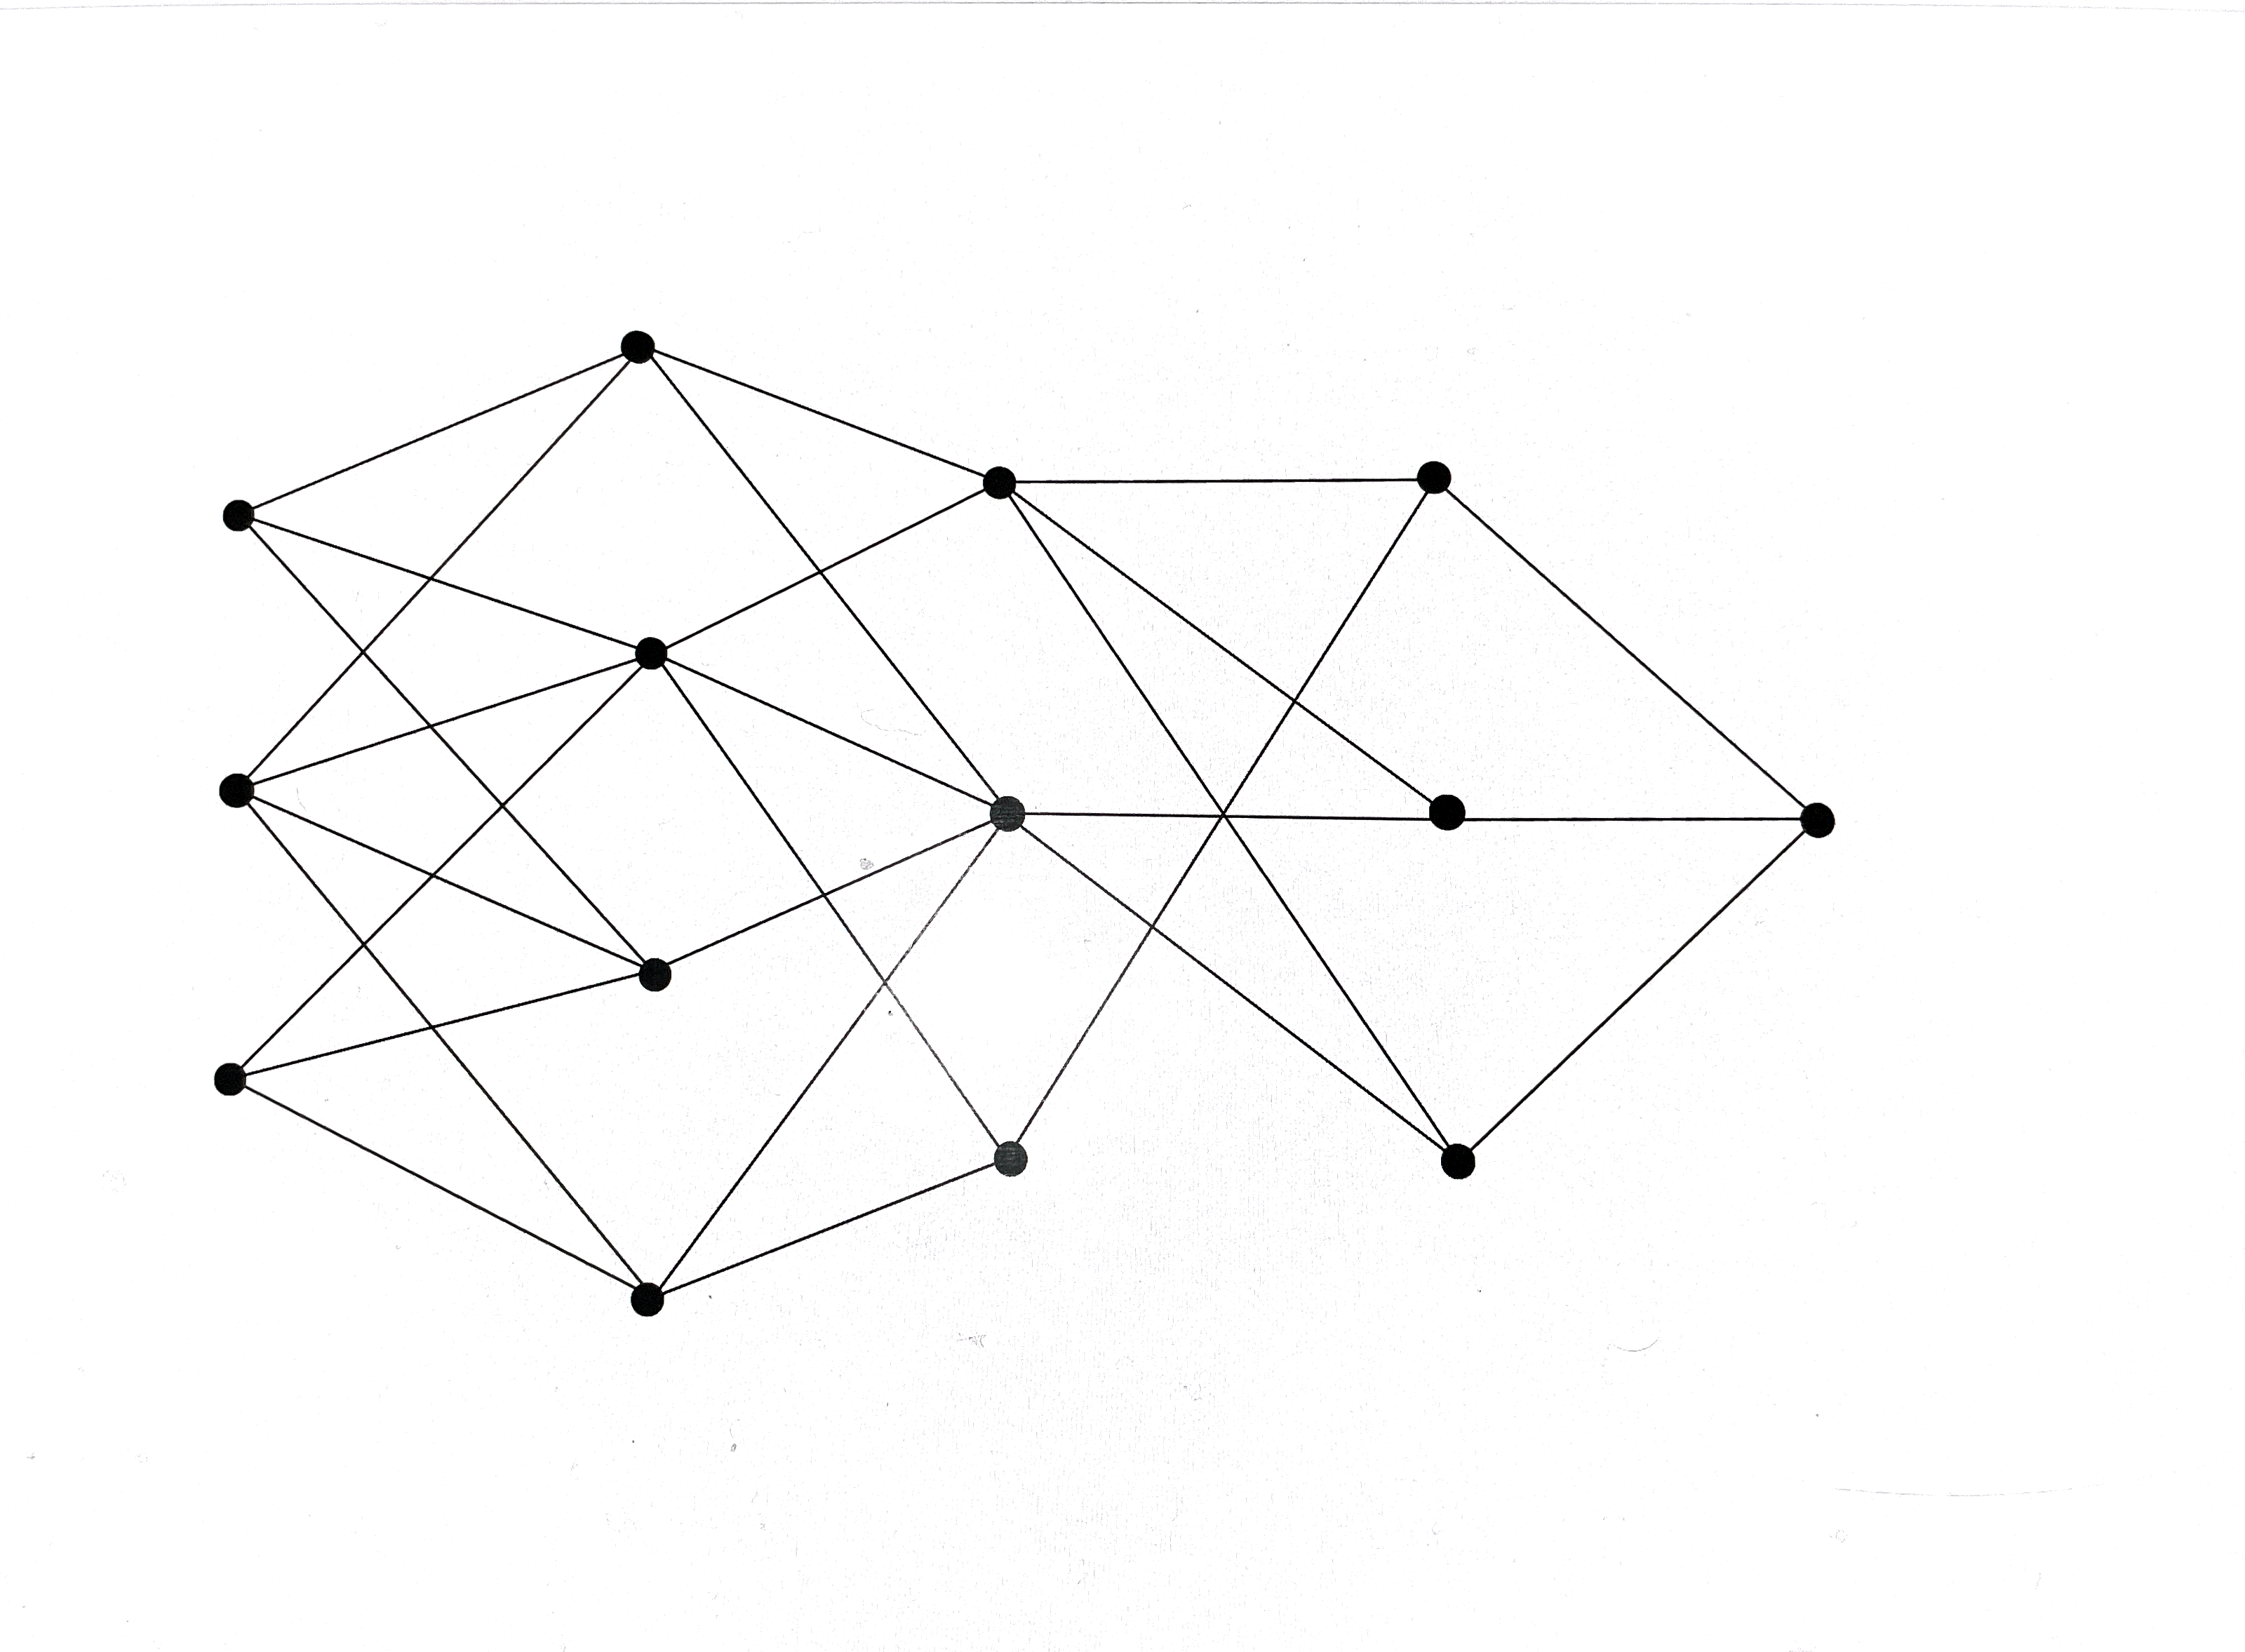
\includegraphics[width=3in]{images/Chapter 10/Weights_Exercice.png}
    \item Find the output of the following neural network for 
    $\vx = \begin{pmatrix}
         1\\
         1\\
         1
        \end{pmatrix}$, 
    $\vb^{(0)} = \begin{pmatrix}
         1\\
         1\\
         1\\
         1
         \end{pmatrix}$
    $\vb^{(1)} = \begin{pmatrix}
         0\\
         \end{pmatrix}$


    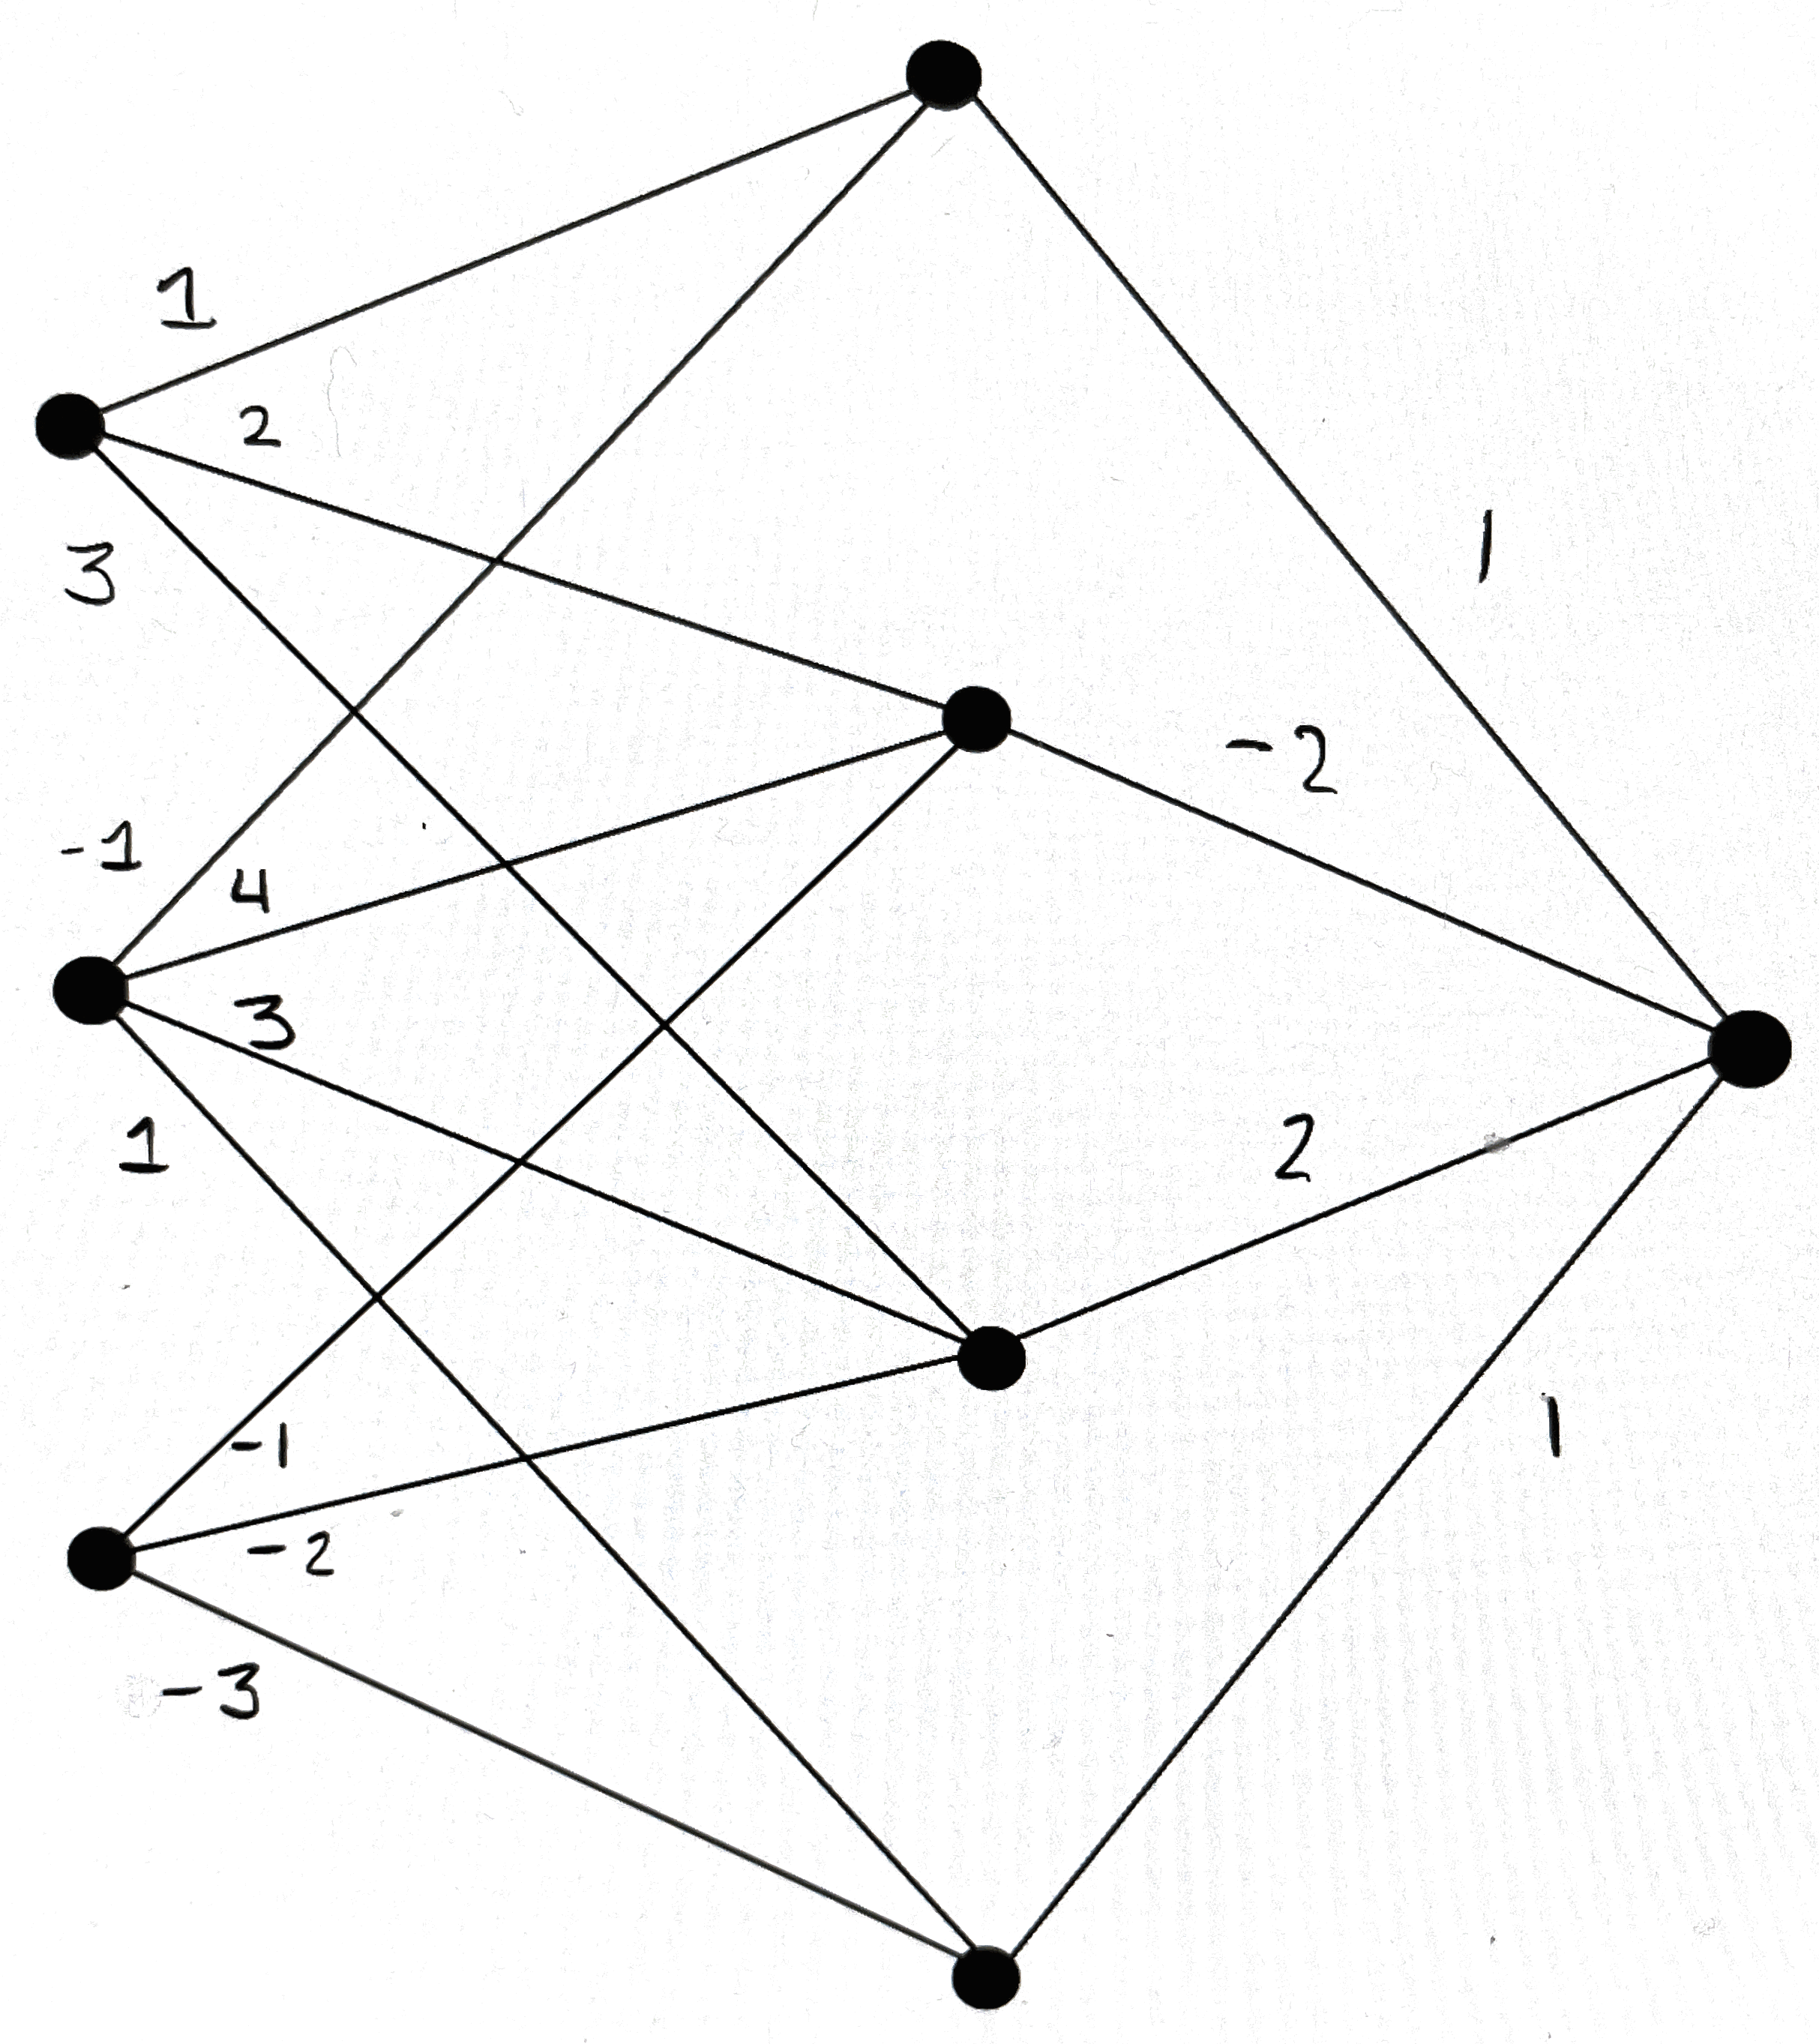
\includegraphics[width=1.5in]{images/Chapter 10/NN_Exercice.png}
    
\end{enumerate}
\section{Solutions to Exercises}
\begin{enumerate}
    \item Start with plugging in the given data matrix in to the sigmoid equation: 
    \begin{equation*}
         sigmoid(XW^{(1)} + \Vec{1}\vb^{(1)}{}^T) = sigmoid \left(
        \begin{pmatrix}
        2 & 1 & 1\\
        0 & 1 & 0\\
        0 & -3 & 2\\
        2 & -2 & 2
        \end{pmatrix} 
        \begin{pmatrix}
         0.5 & 1 & 2\\
         1 & 2 & 0.5\\
         2 & 0.5 & 1
        \end{pmatrix} + 
        \begin{pmatrix}
        1 & 0 & 1\\
        1 & 0 & 1\\
        1 & 0 & 1\\
        1 & 0 & 1
        \end{pmatrix} \right)
    \end{equation*}
    \begin{equation*}
            =sigmoid
            \begin{pmatrix}
                5 & 4.5 & 6.5\\
                2 & 2 & 1.5\\
                2 & -5 & 1.5\\
                4 & -1 & 6
            \end{pmatrix}
            =
            \begin{pmatrix}
                0.73 & 0.99 & 1.00\\
                0.88 & 0.88 & 0.82\\
                0.88 & 0.01 & 0.82\\
                0.98 & 0.27 & 1.00
            \end{pmatrix}
        \end{equation*}
        \begin{equation*}
         ReLU(XW^{(2)} + \Vec{1}\vb^{(2)}{}^T) = ReLU \left(
        \begin{pmatrix}
                0.73 & 0.99 & 1.00\\
                0.88 & 0.88 & 0.82\\
                0.88 & 0.01 & 0.82\\
                0.98 & 0.27 & 1.00
        \end{pmatrix} 
        \begin{pmatrix}
         1 & 2 & 0.5\\
         1 & 2 & 0.5\\
         1 & 2 & 0.5
        \end{pmatrix} + 
        \begin{pmatrix}
        1 & 1 & 1\\
        1 & 1 & 1\\
        1 & 1 & 1\\
        1 & 1 & 1
        \end{pmatrix} \right)
    \end{equation*}
    \begin{equation*}
            =ReLU
            \begin{pmatrix}
                3.72 & 6.44 & 2.36\\
                3.58 & 6.16 & 2.29\\
                2.71 & 4.42 & 1.86\\
                3.25 & 5.5 & 2.13
            \end{pmatrix}
            =
            \begin{pmatrix}
                1 & 1 & 1\\
                1 & 1 & 1\\
                1 & 1 & 1\\
                1 & 1 & 1
            \end{pmatrix}
    \end{equation*}
    The final output is 
        $\begin{pmatrix}
        h_1\\
        h_2\\
        h_3\\
        h_4
        \end{pmatrix}$ $W^{(3)}$ 
    + $\vb^{(3)}$.
    \begin{equation*}
         sigmoid(XW^{(3)} + \Vec{1}\vb^{(3)}{}^T) = sigmoid \left(
        \begin{pmatrix}
                1 & 1 & 1\\
                1 & 1 & 1\\
                1 & 1 & 1\\
                1 & 1 & 1
        \end{pmatrix} 
        \begin{pmatrix}
         1\\
         0.5\\
         2
        \end{pmatrix} + 
        \begin{pmatrix}
        0\\
        1\\
        1\\
        0
        \end{pmatrix} \right)
    \end{equation*}
    \begin{equation*}
            =sigmoid
            \begin{pmatrix}
                3.5\\
                4.5\\
                4.5\\
                3.5
            \end{pmatrix}
            =
            \begin{pmatrix}
                0.97\\
                0.99\\
                0.99\\
                0.97
            \end{pmatrix}
    \end{equation*}
    \item The line extension of the given poset is:
        \begin{center}
            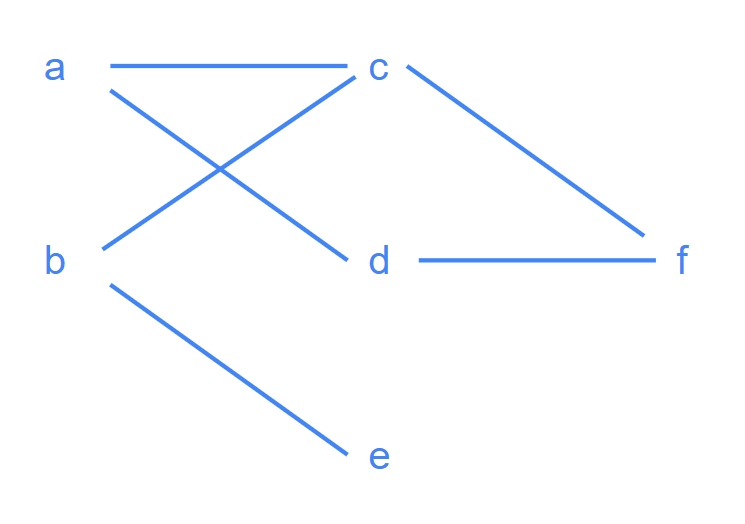
\includegraphics[width=2in]{images/Chapter 10/convention.png}
        \end{center}
    \item The reason why we choose to use sigmoid activation function is because the gradient is 0 when ${\vv^T}$h + ${\vb}$ outside the unit interval. Gradient equals to 0 means there's no direction to improve the parameter.
    \item
    $$
            W^{(0)} = \begin{pmatrix}
                1 & 1 & 0\\
                1 & 1 & 1\\
                1 & 1 & 1\\
                0 & 1 & 1
            \end{pmatrix},
            W^{(1)} = \begin{pmatrix}
                1 & 1 & 0 & 0\\
                1 & 1 & 1 & 1\\
                0 & 1 & 0 & 1\\
            \end{pmatrix},
            W^{(2)} = \begin{pmatrix}
                1 & 0 & 1\\
                1 & 1 & 1\\
                1 & 1 & 0\\
            \end{pmatrix},
            W^{(3)} = \begin{pmatrix}
                1 & 1 & 1\\
            \end{pmatrix}
 $$
\end{enumerate}

\section{Output Neural}
\begin{definition}
  Given a neural network  $N=(H, F, G)$  with depth  $D$ , for  $\vec{x} \in \mathbb{R}^{\# P_{0}} \cong V_{P}^{(0)}$  (an input vector), the hidden features associcted to  $\vec{x}$  at layer  $i$  are
$$
H F_{N}^{(i)} \vec{x}=G_{i} F_{i-1} \ldots F_{1} G_{1} F_{0} \vec{x}
$$
where  $ H F_{N}^{(0)} \vec{x}=\vec{x}$.  
\end{definition}


\begin{figure}[ht]
\centering
\begin{tikzpicture}
    \node[inputNode, thick] (i1) at (0, 0.5) {};
    \node[inputNode, thick] (i2) at (0, 0) {};
    \node[inputNode, thick] (i3) at (0, -0.5) {};
	
    \node[inputNode, thick] (h11) at (2, 1.25) {};
    \node[inputNode, thick] (h12) at (2, 0.75) {};
    \node[inputNode, thick] (h13) at (2, 0.25) {};
    \node[inputNode, thick] (h14) at (2, -0.25) {};
    \node[inputNode, thick] (h15) at (2, -0.75) {};
    \node[inputNode, thick] (h16) at (2, -1.25) {};

    
    \node[inputNode, thick] (h21) at (4, 1) {};
    \node[inputNode, thick] (h22) at (4, 0.5) {};
    \node[inputNode, thick] (h23) at (4, 0) {};
    \node[inputNode, thick] (h24) at (4, -0.5) {};
    \node[inputNode, thick] (h25) at (4, -1) {};

    \node[inputNode, thick] (h41) at (6, 1) {};
    \node[inputNode, thick] (h42) at (6, 0.5) {};
    \node[inputNode, thick] (h43) at (6, 0) {};
    \node[inputNode, thick] (h44) at (6, -0.5) {};
    \node[inputNode, thick] (h45) at (6, -1) {};

    \node[inputNode, thick] (h31) at (8, 1) {};
    \node[inputNode, thick] (h32) at (8, 0.5) {};
    \node[inputNode, thick] (h33) at (8, 0) {};
    \node[inputNode, thick] (h34) at (8, -0.5) {};
    \node[inputNode, thick] (h35) at (8, -1) {};
	\node[inputNode, thick] (o) at (10, 0) {};
    \node[left=1em of h23, align=center] (t12) {$\cdots$}; 
    \node[right=1em of h23, align=center] (t11) {$\cdots$}; 
    \node[left=2.5em of i2, align=center] (t2) {$\vec{x}$}; 
    \node[above=0.5em of h11, align=center] (t3) {$HF_N\vec x$};     
    \node[above=0.5em of h21, align=center] (t4) {$HF_N^{(i)}\vec x$};   
    \node[above=0.5em of h41, align=center] (t5) {$HF_N^{(D-1)}\vec x$};  
    \node[above=0.5em of h31, align=center] (t5) {$HF_N^{(D)}\vec x$};  
    \draw[stateTransition] (0.5,0) -- (1.5, 0);
    \draw[stateTransition] (6.5,0) -- (7.5, 0);
    \draw[stateTransition] (8.5,0) -- (9.5, 0);
    \draw[stateTransition] (-1, 0.5) -- (i1);
    \draw[stateTransition] (-1, 0)   -- (i2);
    \draw[stateTransition] (-1, -0.5)-- (i3);
    \draw[stateTransition] (o) -- node[above] {$\hat{y}$} (11, 0);
    \node[above=of h21, align=center] (l2) {Hidden \\ layer};
    \node[left=7.9em of l2, align=center] (l1) {Input \\ layer};
    \node[right=10em of l2, align=center] (l3) {Output \\ layer};
\end{tikzpicture}
\end{figure}
So the output neural are responsible for predicting the target from  $H F_{N}^{(D-1)} \vec{x}$ . The choice of activation at the output layer depends on the type of targets possible
(i.e. on  $  p_{\text {data }}(\vec{y})$)

 \begin{example}
     \begin{align*}
\text{Input: }&\vec{x}= \text{ (some statistics on two sports teams) }\\
&y=\left\{\begin{array}{ll}0 & \text { if } \operatorname{team} 1 \text { wins } \\ 1 & \text { if } \operatorname{team} 2 \text { wins }\end{array}\right.
\end{align*}

Dataset  $X, \vec{y}$  of previous result. Goal: predict winners of upcoming games.


Idea: Apply a neural network  $N$  so that
$$
N \vec{x}=p(y=1 \mid \vec{x})
$$

\begin{figure}[ht]
\centering
\begin{tikzpicture}
    \node[inputNode, thick] (i1) at (0, 0.5) {};
    \node[inputNode, thick] (i2) at (0, 0) {};
    \node[inputNode, thick] (i3) at (0, -0.5) {};
	
    \node[inputNode, thick] (h11) at (2, 1.25) {};
    \node[inputNode, thick] (h12) at (2, 0.75) {};
    \node[inputNode, thick] (h13) at (2, 0.25) {};
    \node[inputNode, thick] (h14) at (2, -0.25) {};
    \node[inputNode, thick] (h15) at (2, -0.75) {};
    \node[inputNode, thick] (h16) at (2, -1.25) {};

    
    \node[inputNode, thick] (h21) at (4, 1) {};
    \node[inputNode, thick] (h22) at (4, 0.5) {};
    \node[inputNode, thick] (h23) at (4, 0) {};
    \node[inputNode, thick] (h24) at (4, -0.5) {};
    \node[inputNode, thick] (h25) at (4, -1) {};

    \node[inputNode, thick] (h41) at (6, 1) {};
    \node[inputNode, thick] (h42) at (6, 0.5) {};
    \node[inputNode, thick] (h43) at (6, 0) {};
    \node[inputNode, thick] (h44) at (6, -0.5) {};
    \node[inputNode, thick] (h45) at (6, -1) {};

    \node[inputNode, thick] (h31) at (8, 1) {};
    \node[inputNode, thick] (h32) at (8, 0.5) {};
    \node[inputNode, thick] (h33) at (8, 0) {};
    \node[inputNode, thick] (h34) at (8, -0.5) {};
    \node[inputNode, thick] (h35) at (8, -1) {};
	\node[inputNode, thick] (o) at (10, 0) {};
    \node[left=1em of h23, align=center] (t12) {$\cdots$}; 
    \node[right=1em of h23, align=center] (t11) {$\cdots$}; 
    \node[left=2.5em of i2, align=center] (t2) {$\vec{x}$}; 
    \node[above=0.5em of h11, align=center] (t3) {$HF_N\vec x$};     
    \node[above=0.5em of h21, align=center] (t4) {$HF_N^{(i)}\vec x$};   
    \node[above=0.5em of h41, align=center] (t5) {$HF_N^{(D-1)}\vec x$};  
    \node[above=0.5em of h31, align=center] (t5) {$HF_N^{(D)}\vec x$};  
    \draw[stateTransition] (0.5,0) -- (1.5, 0);
    \draw[stateTransition] (6.5,0) -- (7.5, 0);
    \draw[stateTransition] (8.5,0) -- (9.5, 0);
    \draw[stateTransition] (-1, 0.5) -- (i1);
    \draw[stateTransition] (-1, 0)   -- (i2);
    \draw[stateTransition] (-1, -0.5)-- (i3);

    \draw[stateTransition] (o) -- (11, 1)  node[right] {$>.S$ team 1 wins};
    \draw[stateTransition] (o) -- (11, -1)  node[right] {$<.S$ team 2 wins};

    \node[above=of h21, align=center] (l2) {Hidden \\ layer};
    \node[left=8em of l2, align=center] (l1) {Input \\ layer};
    \node[right=10em of l2, align=center] (l3) {Output \\ layer};
\end{tikzpicture}
\end{figure}
Sigmoid activation makes sense here.
\end{example}

% \newpage
% \begin{figure}[ht]
% \centering
% \begin{tikzpicture}
%     \node[inputNode, thick] (i1) at (0, 0.5) {};
%     \node[inputNode, thick] (i2) at (0, 0) {};
%     \node[inputNode, thick] (i3) at (0, -0.5) {};
	
%     \node[inputNode, thick] (h11) at (2, 1.25) {};
%     \node[inputNode, thick] (h12) at (2, 0.75) {};
%     \node[inputNode, thick] (h13) at (2, 0.25) {};
%     \node[inputNode, thick] (h14) at (2, -0.25) {};
%     \node[inputNode, thick] (h15) at (2, -0.75) {};
%     \node[inputNode, thick] (h16) at (2, -1.25) {};

    
%     \node[inputNode, thick] (h21) at (4, 1) {};
%     \node[inputNode, thick] (h22) at (4, 0.5) {};
%     \node[inputNode, thick] (h23) at (4, 0) {};
%     \node[inputNode, thick] (h24) at (4, -0.5) {};
%     \node[inputNode, thick] (h25) at (4, -1) {};

%     \node[inputNode, thick] (h41) at (6, 1) {};
%     \node[inputNode, thick] (h42) at (6, 0.5) {};
%     \node[inputNode, thick] (h43) at (6, 0) {};
%     \node[inputNode, thick] (h44) at (6, -0.5) {};
%     \node[inputNode, thick] (h45) at (6, -1) {};

%     \node[inputNode, thick] (h31) at (8, 1) {};
%     \node[inputNode, thick] (h32) at (8, 0.5) {};
%     \node[inputNode, thick] (h33) at (8, 0) {};
%     \node[inputNode, thick] (h34) at (8, -0.5) {};
%     \node[inputNode, thick] (h35) at (8, -1) {};
% 	\node[inputNode, thick] (o) at (10, 0) {};
%     \node[left=1em of h23, align=center] (t12) {$\cdots$}; 
%     \node[right=1em of h23, align=center] (t11) {$\cdots$}; 
%     \node[left=2.5em of i2, align=center] (t2) {$\vec{x}$}; 
%     \node[above=0.5em of h11, align=center] (t3) {$HF_N\vec x$};     
%     \node[above=0.5em of h21, align=center] (t4) {$HF_N^{(i)}\vec x$};   
%     \node[above=0.5em of h41, align=center] (t5) {$HF_N^{(D-1)}\vec x$};  
%     \node[above=0.5em of h31, align=center] (t5) {$HF_N^{(D)}\vec x$};  
%     \draw[stateTransition] (0.5,0) -- (1.5, 0);
%     \draw[stateTransition] (6.5,0) -- (7.5, 0);
%     \draw[stateTransition] (8.5,0) -- (9.5, 0);
%     \draw[stateTransition] (-1, 0.5) -- (i1);
%     \draw[stateTransition] (-1, 0)   -- (i2);
%     \draw[stateTransition] (-1, -0.5)-- (i3);

%     \node[above=of h21, align=center] (l2) {Hidden \\ layer};
%     \node[left=8em of l2, align=center] (l1) {Input \\ layer};
%     \node[right=10em of l2, align=center] (l3) {Output \\ layer};
% \end{tikzpicture}
% \end{figure}
% $$
% \vec{x}^{(i)}=H F_{N}^{i}(\vec{x})=G^{(i)} F^{(i-1)} \ldots G^{(1)} F_{\Delta}^{(0)} \vec{x}
% $$

\begin{example}
 Input  $\vec{x}$  statstics on sports teams  1 \& 2 
$$
y=\left\{\begin{array}{rc}
1 & \text { team } 1 \text { wins } \\
0 & \text { team } 2 \text { wins }
\end{array}\right.
$$
Idea: want  $N \vec{x}=p(y=1 \mid \vec{x})$ 

\begin{figure}[ht]
\centering
\begin{tikzpicture}
    \node[inputNode, thick] (i1) at (0, 0.5) {};
    \node[inputNode, thick] (i2) at (0, 0) {};
    \node[inputNode, thick] (i3) at (0, -0.5) {};
	
    \node[inputNode, thick] (h11) at (2, 1.25) {};
    \node[inputNode, thick] (h12) at (2, 0.75) {};
    \node[inputNode, thick] (h13) at (2, 0.25) {};
    \node[inputNode, thick] (h14) at (2, -0.25) {};
    \node[inputNode, thick] (h15) at (2, -0.75) {};
    \node[inputNode, thick] (h16) at (2, -1.25) {};

    
    \node[inputNode, thick] (h21) at (4, 1) {};
    \node[inputNode, thick] (h22) at (4, 0.5) {};
    \node[inputNode, thick] (h23) at (4, 0) {};
    \node[inputNode, thick] (h24) at (4, -0.5) {};
    \node[inputNode, thick] (h25) at (4, -1) {};

    \node[inputNode, thick] (h41) at (6, 1) {};
    \node[inputNode, thick] (h42) at (6, 0.5) {};
    \node[inputNode, thick] (h43) at (6, 0) {};
    \node[inputNode, thick] (h44) at (6, -0.5) {};
    \node[inputNode, thick] (h45) at (6, -1) {};

    \node[inputNode, thick] (h31) at (8, 1) {};
    \node[inputNode, thick] (h32) at (8, 0.5) {};
    \node[inputNode, thick] (h33) at (8, 0) {};
    \node[inputNode, thick] (h34) at (8, -0.5) {};
    \node[inputNode, thick] (h35) at (8, -1) {};
	\node[inputNode, thick] (o) at (10, 0) {};
    \node[left=1em of h23, align=center] (t12) {$\cdots$}; 
    \node[right=1em of h23, align=center] (t11) {$\cdots$}; 
    \node[left=2.5em of i2, align=center] (t2) {$\vec{x}$}; 
  
    \node[above=0.5em of h31, align=center] (t5) {$HF_N^{(D-1)}\vec x=h$};  
    \node[right=0.5em of o, align=center] (t6) {$N\vec x\in[0,1]$};
    \draw[stateTransition] (0.5,0) -- (1.5, 0);
    \draw[stateTransition] (6.5,0) -- (7.5, 0);
    \draw[stateTransition] (8.5,0) -- (9.5, 0);
    \draw[stateTransition] (-1, 0.5) -- (i1);
    \draw[stateTransition] (-1, 0)   -- (i2);
    \draw[stateTransition] (-1, -0.5)-- (i3);
\end{tikzpicture}
\end{figure}
Makes sense to use sigmoid activation for  $G^{(D)}$.
\end{example}
\begin{remark}
    This is equvalent  $p$  transforming  $\vec{x}$  to new features  $\vec{h}$  and performing logistic regression on  $\vec{h}$.
\end{remark}

\newpage

\begin{example}
    
$\vec{x}$  statistics about a company $y$ has stock price in 1 week ($y$ has continuous distribution e.g. Gaussian) 


linear activation  $G^{(D)}(y)=y$  makes sense here.

\begin{figure}[ht]
\centering
\begin{tikzpicture}
    \node[inputNode, thick] (i1) at (0, 0.5) {};
    \node[inputNode, thick] (i2) at (0, 0) {};
    \node[inputNode, thick] (i3) at (0, -0.5) {};
	
    \node[inputNode, thick] (h11) at (2, 1.25) {};
    \node[inputNode, thick] (h12) at (2, 0.75) {};
    \node[inputNode, thick] (h13) at (2, 0.25) {};
    \node[inputNode, thick] (h14) at (2, -0.25) {};
    \node[inputNode, thick] (h15) at (2, -0.75) {};
    \node[inputNode, thick] (h16) at (2, -1.25) {};

    \node[inputNode, thick] (h21) at (4, 1) {};
    \node[inputNode, thick] (h22) at (4, 0.5) {};
    \node[inputNode, thick] (h23) at (4, 0) {};
    \node[inputNode, thick] (h24) at (4, -0.5) {};
    \node[inputNode, thick] (h25) at (4, -1) {};

    \node[inputNode, thick] (h41) at (6, 1) {};
    \node[inputNode, thick] (h42) at (6, 0.5) {};
    \node[inputNode, thick] (h43) at (6, 0) {};
    \node[inputNode, thick] (h44) at (6, -0.5) {};
    \node[inputNode, thick] (h45) at (6, -1) {};

    \node[inputNode, thick] (h31) at (8, 1) {};
    \node[inputNode, thick] (h32) at (8, 0.5) {};
    \node[inputNode, thick] (h33) at (8, 0) {};
    \node[inputNode, thick] (h34) at (8, -0.5) {};
    \node[inputNode, thick] (h35) at (8, -1) {};
	\node[inputNode, thick] (o) at (10, 0) {};
    \node[left=1em of h23, align=center] (t12) {$\cdots$}; 
    \node[right=1em of h23, align=center] (t11) {$\cdots$}; 
    \node[left=2.5em of i2, align=center] (t2) {$N\qquad\vec{x}$}; 
  
    \node[above=0.5em of h31, align=center] (t5) {$\vec h$};  
    \draw[stateTransition] (0.5,0) -- (1.5, 0);
    \draw[stateTransition] (6.5,0) -- (7.5, 0);
    \draw[stateTransition] (8.5,0) -- (9.5, 0);
    \draw[stateTransition] (-1, 0.5) -- (i1);
    \draw[stateTransition] (-1, 0)   -- (i2);
    \draw[stateTransition] (-1, -0.5)-- (i3);
\end{tikzpicture}
\end{figure}
\end{example}

\begin{remark}
    This is equivalent to performing linear regression on  $HF_{N}^{(D-1)}(\vec{x})$
\end{remark}

\begin{example}
    $\vec{X}=$  vectorized image of an animals  $\left(\begin{array}{c}k \\ \text { types }\end{array}\right) $
$$
y=\left\{\begin{array}{ll}
e_{1} & \text { if cat } \\
e_{2} & \text { if dog } \\
\vdots & \\
e_{k} & \text { if llama }
\end{array}\right. \in \mathbb{R}^k = \langle e_1,e_2,\cdots,e_k \rangle
$$
(call a one hot encoding)
want $N \vec{x}=\hat{y} \text { where } \hat{y}_{i}=p\left(y=e_{i} \mid \vec{x}\right),  \left(\therefore\sum_{i=1}^{k} \hat{y}_{i}=1\right.$

\begin{figure}[ht]
\centering
\begin{tikzpicture}
    \node[inputNode, thick] (i1) at (0, 0.5) {};
    \node[inputNode, thick] (i2) at (0, 0) {};
    \node[inputNode, thick] (i3) at (0, -0.5) {};
	
    \node[inputNode, thick] (h11) at (2, 1.25) {};
    \node[inputNode, thick] (h12) at (2, 0.75) {};
    \node[inputNode, thick] (h13) at (2, 0.25) {};
    \node[inputNode, thick] (h14) at (2, -0.25) {};
    \node[inputNode, thick] (h15) at (2, -0.75) {};
    \node[inputNode, thick] (h16) at (2, -1.25) {};

    \node[inputNode, thick] (h21) at (4, 1) {};
    \node[inputNode, thick] (h22) at (4, 0.5) {};
    \node[inputNode, thick] (h23) at (4, 0) {};
    \node[inputNode, thick] (h24) at (4, -0.5) {};
    \node[inputNode, thick] (h25) at (4, -1) {};

    \node[inputNode, thick] (h41) at (6, 1) {};
    \node[inputNode, thick] (h42) at (6, 0.5) {};
    \node[inputNode, thick] (h43) at (6, 0) {};
    \node[inputNode, thick] (h44) at (6, -0.5) {};
    \node[inputNode, thick] (h45) at (6, -1) {};

    \node[inputNode, thick] (h31) at (8, 1) {};
    \node[inputNode, thick] (h32) at (8, 0.5) {};
    \node[inputNode, thick] (h33) at (8, 0) {};
    \node[inputNode, thick] (h34) at (8, -0.5) {};
    \node[inputNode, thick] (h35) at (8, -1) {};
	\node (o) at (10, 0) {$\vec y \in \mathbb{R}^k$};
    \node[left=1em of h23, align=center] (t12) {$\cdots$}; 
    \node[right=1em of h23, align=center] (t11) {$\cdots$}; 
    \node[left=2.5em of i2, align=center] (t2) {$N\qquad\vec{x}$}; 
  
    \node[above=0.5em of h41, align=center] (t5) {$\vec h$};  
    \draw[stateTransition] (0.5,0) -- (1.5, 0);
    \draw[stateTransition] (6.5,0) -- (7.5, 0);
    \draw[stateTransition] (-1, 0.5) -- (i1);
    \draw[stateTransition] (-1, 0)   -- (i2);
    \draw[stateTransition] (-1, -0.5)-- (i3);
\end{tikzpicture}
\end{figure}

Define  $G^{(0)}=  \mathrm{softmax}$ where   $\mathrm{softmax}(\vec{h})=\frac{\exp _{p}\left(h_{i}\right)}{\sum_{j=1}^{k} \exp \left(h_{j}\right)}$ 
Softmax makes sense here.
\end{example}

\begin{remark}
    In each case we are choosing an activation function which will give the gradient nice properties. We want the gradient to have the property that when  $W, B$  are far from "local min, the gradient stays sufficiently large, (so GD does not "get stuck").
\end{remark}


\section{Optimization for Neural Networks}
Let  $N$  be a neural network and  $J(W, B)$  a cost function to measure "proximity" between  $N_{\vec{x}}$  and target  $\vec{y}$  on a dataset  $X, Y$ . To run gradient descent to find good values for $W,B$ we need to compute
$$
\frac{\partial J}{\partial W^{(i)}}, \frac{\partial J}{\partial b^{(i)}} \quad 0 \leq i \leq D-1
$$

Definition The signal ost of layer $i$ for input  $\vec{x}$  is
$$
S^{(i)}=F^{(i)} G^{(i)} \ldots G^{(1)} F^{(0)} \vec{x} \quad S^{(0)}=F^{(0)} \vec{x}
$$
\begin{remark}
    $G^{(i+1)} S^{(i)}=H F_{N}^{(i+1)}(\vec{x})=\vec{x}^{(i+1)}$ 
\end{remark}


\begin{example}

$$
\begin{array}{l}
W^{(0)}=\left(\begin{array}{ll}
w_{11}^{0} & w_{12}^{0} \\
w_{21}^{0} & w_{i 2}^{0}
\end{array}\right) \quad \vec{b}^{(0)}=\left(\begin{array}{l}
b_{i}^{i} \\
b_{2}^{0}
\end{array}\right) \\
W^{(1)}=\left(w_{11}^{\prime} w_{12}^{\prime}\right) \quad \vec{b}^{(1)}=\left(b_{1}^{\prime}\right) \\
S^{(0)}=W^{(0)} \vec{x}+\vec{b}^{(0)} \\
\vec{x}^{(1)}=G^{(1)}\left(s^{(0)}\right)=G^{(1)}\left(W^{(0)} \vec{x}+\vec{b}^{(0)}\right) \\
S^{(1)}=W^{(1)} G^{(1)}\left(S^{(0)}\right)+b^{(1)}=W^{(1)} \vec{x}^{(1)}+b^{(1)} \\
\vec{x}^{(2)}=G^{(2)}\left(s^{(1)}\right)=N \vec{x} \\
\end{array}
$$
    \begin{figure}[ht]
\centering
\begin{tikzpicture}
    \node[inputNode, thick] (i1) at (0, 1) {};
    \node[inputNode, thick] (i2) at (0, -1) {};
    \node[inputNode, thick] (h11) at (4, 1) {};
    \node[inputNode, thick] (h12) at (4, -1) {};
    \node[inputNode, thick] (o) at (8, 0) {};
    \node[align=center] (t1) at (-0.5,0) {$\vec{x}$}; 
  
    \draw[stateTransition] (i1) -- (h11);
    \draw[stateTransition] (i1) -- (h12);
    \draw[stateTransition] (i2) -- (h11);
    \draw[stateTransition] (i2) -- (h12);
    \draw[stateTransition] (h11) -- (o);
    \draw[stateTransition] (h12) -- (o);
    
    \node[ align=center] (t1) at (2,1.55) {$S^{(0)}$}; 
    \node[ align=center] (t2) at (6,1) {$S^{(1)}$};
    \node[above=0em of i1, align=center] (t3) {$\vec x$}; 
    \node[above=0em of h11, align=center] (t4) {$\vec x^{(1)}$}; 
    \node[right=0em of o, align=center] (t5) {$\vec x^{(2)}=N\vec x$};

    \draw[stateTransition] (0.2,1.5) -- node[above]{$F^{(0)}$} (1.7,1.5);
    \draw[stateTransition] (2.2,1.5) -- node[above]{$G^{(0)}$} (3.7,1.5);

    \draw[stateTransition] (4.2,1.4) -- node[above]{$F^{(1)}$} (5.7,1);
    \draw[stateTransition] (6.2,0.8) -- node[above]{$G^{(1)}$} (8.5,0.2);
\end{tikzpicture}
\end{figure}
Cost function  $J(W, B)=\sum_{i=1}^{m} L\left(N \vec{x}_{i}, \vec{y}_{i}\right) $. 
Need to find derivetives of  $L(N \vec{x}, \vec{y})$ 
\end{example}

\begin{remark}
    $\displaystyle\frac{\partial}{\partial v}(f \circ g)(v)=\left.\frac{\partial f(w)}{\partial w}\right|_{w=g(v)} \frac{\partial}{\partial v} g(v) $
$$
\text { where }\left.\frac{\partial f(w)}{\partial w}\right|_{w=g(v)}=\frac{\partial f}{\partial g(v)}
$$
\end{remark}

\section{Backpropagation}

Backpropagation is the algorithm we use to train feed forward neural networks. This algorithm efficiently computes the gradient of the loss function with respect to the weights of the network, adjusting the weights and biases of the model. This allows us to use gradient descent or stochastic gradient descent methods to train multilayer networks, updating weights to minimize loss.


We will explore backpropagation for a network defined by the poset $P(n_{0},n_{1},...n_{D})$, i.e., each layer is fully connected to adjacent layers, dataset $X\in\R^{m\times n}, Y\in\R^{m\times k}$ and a loss function
$$J(W,B)=\frac{1}{m}\sum_{i=1}^{m}L(N\vx_{i},\vy_{i})$$

\medskip
Now, let's find expressions for $\delta$, so we may use them to find expressions for the gradient of the loss function.
\begin{ceqn}
    \begin{align*}
        \delta^{(D-1)}&=\frac{\partial L}{\partial S^{(D-1)}}=\frac{\partial L}{\partial N\vx_{i}}\cdot\frac{\partial N\vx_{i}}{\partial S^{(D-1)}} \\
        &=\frac{\partial L}{\partial N\vx_{i}}\cdot\frac{\partial G^{(D)}}{\partial S^{(D-1)}}
    \end{align*}
\end{ceqn}
\begin{remark}
    Use $N\vx=G^{(D)}S^{(D-1)}$
\end{remark}
\smallskip
and for $0\leq l<D-1$:
\begin{ceqn}
\begin{align*}
    \delta^{(l)}&=\frac{\partial L}{\partial S^{(l)}}=\frac{\partial L}{\partial S^{(l+1)}}\cdot\frac{\partial S^{(l+1)}}{\partial S^{(l)}}\\
&=\delta^{(l+1)}W^{(l+1)}\frac{\partial G^{(l+1)}}{\partial S^{(l)}}
\end{align*}
\end{ceqn}
\begin{remark}
    Use $S^{(l+1)} = W^{(l+1)}G^{(l+1)}S^{(l+1)} + b^{(l+1)}$
\end{remark}
\medskip
With these handy values, we can now calculate:
\begin{ceqn}
\begin{align*}
    \frac{\partial L}{\partial W^{(l)}} &= \frac{\partial L}{\partial S^{(l)}}\cdot\frac{\partial S^{(l)}}{\partial W^{(l)}} \\
    &= \sum_{k=1}^{n_{l+1}}{\frac{\partial L}{\partial S_{k}^{(l)}}\cdot\frac{\partial S_{k}^{(l)}}{\partial W^{(l)}}} \\
    &= \sum_{k,j}{\delta_{k}^{(l)}\sum_{j=1}^{n_{l}}{\ME_{kj}\vx_{j}^{(l)}}} \\
    &= \sum_{k=1}^{n_{l+1}}{\delta_{k}^{(l)}\vx_{j}^{(l)}\ME_{kj}} \\
    &= \mathrm{outer}(\delta^{(l)},\vx^{(l)})
\end{align*}
\end{ceqn}

\begin{remark}
    Use $S_{k}^{(l)}=\sum_{j=1}^{n_l}{W_{k,j}^{(l)}x_j^{(l)}}+b_k^{(l)}$ \\
    Note that $\frac{\partial}{\partial W^{(l)}}W_{k,j}^{(l)}=\ME_{kj}$ where $\ME_{kj}$ is a matrix with an entry 1 in $(k,j)$ and zeros elsewhere.
\end{remark}

\smallskip
Similarly, we calculate:

\begin{ceqn}
\begin{align*}
    \frac{\partial L}{\partial b^{(l)}} &= \frac{\partial L}{\partial S^{(l)}}\cdot\frac{\partial S^{(l)}}{\partial b^{(l)}} \\
    &= \frac{\partial L}{\partial S^{(l)}} \\
    &= \delta^{(l)}
\end{align*}
\end{ceqn}

\medskip
Equipped with these partial derivatives with respect to the weight and bias matrices, we can now calculate the gradient for our arbitrary loss function:

$$J(W,B)=\frac{1}{m}\sum_{i=1}^{m}L(N\vx_{i},\vy_{i})$$

$$\frac{\partial J}{\partial W^{(l)}}=\frac{1}{m}\sum_{i=1}^{m}{\mathrm{outer}(\delta_{i}^{(l)},\vx_{i}^{(l)})}$$

$$\frac{\partial J}{\partial b^{(l)}}=\frac{1}{m}\sum_{i=1}^{m}\delta_{i}^{(l)}$$

\section{Regularization}

As we have learned with previous models, we do not want to train our feed forward neural network in such a way that the model is overfitted or underfitted. As such, we can use regularization to calibrate our model and minimize loss.

Let's consider stochastic gradient descent, a variant of gradient descent where only a few samples are selected randomly per iteration, instead of the complete data. We can take a look at the algorithm we use for each step:

\begin{algorithm}
    \caption{Regularization for Stochastic Gradient Descent Step}
    \begin{algorithmic}[1]
            \State Pick $\alpha > 0$
            \State Pick an arbitrary batch $Ba$
            \State Approximate $J(W,B)=\frac{1}{|Ba|}\sum_{i\in Ba}L(N\vx_{i},\vy_{i})$ and append to list of costs
		\For {$i \in Ba$}
        \State Compute [$(\vx_{i}^{(0)}, \S_{i}^{(0)}),\ldots,(\vx_{i}^{(D-1)}, \S_{i}^{(D-1)}),(\vx_{i}^{(D)})$]
        \State Compute [$\delta_{i}^{(D-1)},\ldots,\delta_{i}^{(0)}$]
        \State Compute $\frac{\partial J}{\partial W^{(l)}}=\frac{1}{|Ba|}\sum_{i\in Ba}{\mathrm{outer}(\delta_{i}^{(l)},\vx_{i}^{(l)})}$
		\State Compute $\frac{\partial J}{\partial b^{(l)}}=\frac{1}{|Ba|}\sum_{i \in Ba}\delta_{i}^{(l)}$
		\EndFor		
		\For {$l$ in range($D$)}
        \State $W^{(l)}= W^{(l)} - \alpha \frac{\partial J}{\partial W^{(l)}}$
        \State $b^{(l)}= b^{(l)} - \alpha \frac{\partial J}{\partial b^{(l)}}$
		\EndFor        
	\end{algorithmic} 
\end{algorithm}

If the correct neural network architecture is used, stochastic gradient descent can be used to find weights and biases that provide good performance on training and testing data.

\section{Common Loss Functions}

There are multiple loss (cost) functions we can use to train a feed forward neural network. Let's take a look at a few commonly used functions:

\smallskip
\begin{definition}
    \define{Square Error Loss} is defined by
    $$
    L_{SE}(N\vx,\vy) = ||N\vx-\vy||_{2}^{2}
    $$
\end{definition}
Square Error Loss is mostly used for linear regression, and is one of the simplest loss functions. The function ensures that the trained model has no outliers with huge errors, since a larger weight is assigned to such errors (thanks to the squaring part of the function).

\medskip
\begin{definition}
    \define{Cross Entropy Loss} is defined by
    \begin{ceqn}
    \begin{align*}
        L_{CE}(N\vx,\vy) &= -\vy^\intercal Log(N\vx) \\
        &= -\sum_{i=1}^{n_D}{\vy_i\log((N\vx)_i)}
    \end{align*}
    \end{ceqn}
\end{definition}
Cross Entropy Loss is used for multiclass classifiers which use softmax output neurons.

\medskip
\begin{definition}
    \define{Binary Cross Entropy Loss} is defined by
    $$
    L_{BCE}(N\vx,\vy) = -\vy^\intercal\log(N\vx) - (1-\vy)\log(1-N\vx)
    $$
\end{definition}
As its name suggests, Binary Cross Entropy Loss is used for binary classifiers, which use sigmoid output neurons.


\section{Vanishing Gradient Problem}
In practice, the function of a neural network N is non-convex, so there may be flat regions one may "get stuck" in during (stuck-stic) gradient descent.

\begin{center}
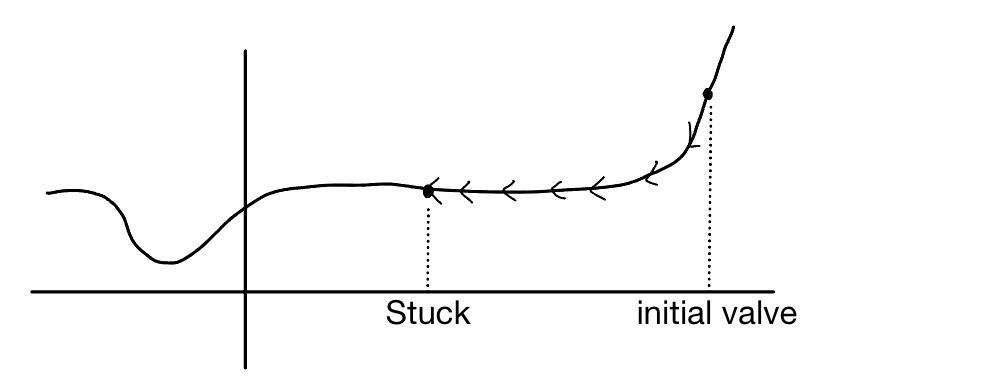
\includegraphics[width=4in]{images/Chapter 10/10.5(1).png}

\end{center}

\begin{remark}
Factors that affect the "flatness" of cost function:
\item 1. Choice of the loss function: $$
\begin{cases}
        SE & \text {lot of flat regions} \\
        CE & \text {less flat regions} \\
        BCE & \text {least of flat regions}
        \end{cases}
$$
2. Choice of activation(the ones we discussed so fare are good choices)

Note: Using several sigmoids in hidden layers can cause flatness.

Suggestion: Use ReLu in hidden layers

3. Momentum

4. Weight Initialization

\end{remark}


\subsection{Momentum Method}
Motivation(from physics). Momentum is one of the most popular techniques used to improve the speed of convergence of the Gradient Descent algorithm.

Consider a ball rolling on a surface

\begin{center}
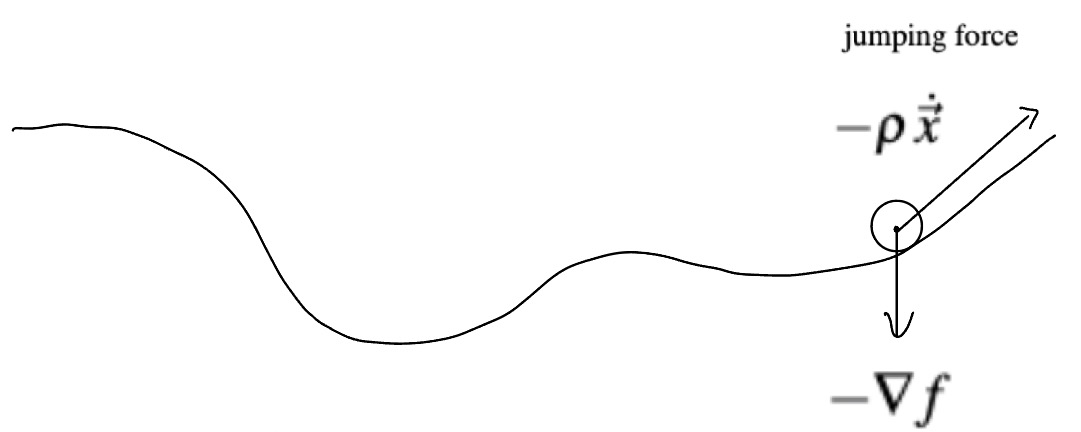
\includegraphics[width=4in]{images/Chapter 10/10.5(2).png}

\end{center}

$$\text {f = potential function,  } {f\,({\vec{x})=m\,g\,x_3}}$$

$$\sum{\vec{F}\,=\,m\,\vec{a}\,\Longrightarrow\,\ddot{\vec{x}}}\,=\,\rho\,\dot{\vec{x}}\,-\,\nabla{f}(\vec{x})$$


To solve: Express as a system of First order ODEs
$$
\dot{\vec{V}}\,=\,-\rho\,\vec{v}\,-\,\nabla{f}(\vec{x})$$
$$\dot{\vec{x}}\,=\,\vec{V}$$

Write this as a finite difference system
(Pick $\nabla{t}$ small enough so that $\rho\,\nabla{t}\,<\,1$)
$$
\vec{V}_{n+1}\,-\,\vec{V}_n\,=-\rho\,\vec{V}_n\,\nabla{t}\,-\,\nabla{f(\vec{x}_n)}\,\nabla{t}
$$
$$
\vec{X}_{n+1}\,-\,\vec{X}_n\,=\,\vec{V}_{n+1}\,\nabla{t}
$$

Let $\epsilon\,=\,\nabla{t}\,$,$\,\,\mu\,=1-\rho\,\epsilon\,$ with$\,\,\,0\leq\mu\,<\,1$
$$
\vec{V}_{n+1}\,=\,\mu\,\vec{V}_n\,-\,\epsilon\,\nabla{f(\vec{x}_n)}
$$
$$
\vec{X}_{n+1}\,=\,\vec{X}_n\,+\,\epsilon\,\vec{V}_{n+1}
$$

let $\vec{V}\,\epsilon\,=\Tilde{\vec{V}}\,\,\,\text{(new scale for velocity)}$
$$
\frac{\tilde{\vec{V}}_{n+1}}{\epsilon}\,=\frac{\mu\,\tilde{\vec{V}}_{n}}{\epsilon}\,-\,\epsilon\,\nabla{f(\vec{x}\,n)}
$$

Define $\alpha\,=\,\epsilon^2$
$$
\tilde{\vec{V}}_{n+1}\,=\,\mu\,\tilde{\vec{V}}_n\,-\,\alpha\,\nabla{f(\vec{x}\,n)}$$
$$
\vec{X}_{n+1}\,=\,\vec{X}_n\,+\,\tilde{\vec{V}}_{n+1}$$

if $\mu=0$, this is just a gradient descent

\begin{example}
The problem with gradient descent is that the weight update at a moment (t) is governed by the learning rate and gradient at that moment only. It doesn’t take into account the past steps taken while traversing the cost space.
$$\nabla{w(t)}\,=\,-\eta\delta(t)$$
The gradient of the cost function at saddle points( plateau) is negligible or zero, which in turn leads to small or no weight updates. Hence, the network becomes stagnant, and learning stops.
(a) How can momentum fix this?


Solution: Imagine you have a ball rolling from point A. The ball starts rolling down slowly and gathers some momentum across the slope AB. When the ball reaches point B, it has accumulated enough momentum to push itself across the plateau region B and finally follow slope BC to land at the global minima C.

(b) How can this be used and applied to Gradient Descent?


Solution: To account for the momentum, we can use a moving average over the past gradients. In regions where the gradient is high like AB, weight updates will be large. Thus, in a way we are gathering momentum by taking a moving average over these gradients. But there is a problem with this method, it considers all the gradients over iterations with equal weight-age. The gradient at t=0 has equal weight-age as that of the gradient at the current iteration t. We need to use some sort of weighted average of the past gradients such that the recent gradients are given more weight-age.

\end{example}



\subsection{Weight Initialization}
Weight initialization is an important consideration in the design of a neural network model.

~\\Neural network models are fit using an optimization algorithm called stochastic gradient descent that incrementally changes the network weights to minimize a loss function, hopefully resulting in a set of weights for the mode that is capable of making useful predictions.

~\\The nodes in neural networks are composed of parameters referred to as weights used to calculate a weighted sum of the inputs.
Neural net performance depends heavily an $W^{(l)}$ weight initialization \underline{especially} if D is large. Depends less on bias initialization $b^{(l)}$ but this depends on architecture.

~\\\textbf{Claim}: 
\textcircled{1} If the initialized values of $W^{(l)}$ are too small, the variance of $J^{(l)}$ decreases at each layer 
\textcircled{2} If initialized weights are too large, variance $s^{(l)}$ amplifies at each layer.


\subsection{Xavier Initialization} Based on the assumption that Var($s^{(\lambda)}$ should remain constant at each layer.

For P($n_{0}$,...,$n_{0}$) entries of $W^{(l)}$ should be sampled from $N(x;0,\frac{2}{n_{l-1}+n_{l}})$.

~\\Many other "suggestions" exist

- Read section 8.4 of the Deep Learning book

- Read section 6.3 of the Deep Learning Architectures

Bias can usually be initialized to $\vec{O}$ \par


~\\\underline{A way to do SGD on neural net N} (for P($n_{0},...,n_{0}$))\\

Pick $\alpha_{step size}$\textless{0}, $\lambda_{reg-parameter}$\textless{0}, $\mu_{momentum}$\textless{0}, max\_iters, batch\_size


For $0\leq {l} \leq D-1$ initialize $W^{(l)}$ by sampling $N(x;0,\frac{2}{n_{l-1}+n_{l}})$
$b^{(o)} = \vec{(O)}$

\hspace{3cm}{initialize $V_{w}^{(l)} = np.zeros(W^{(l)}.shape)$

\hspace{3cm}$V_{b}^{(l)} = np.zeros(b^{(l)}.shape)$}

$epochs = 0$\\

While epochs \textless{max\_iters}:

\hspace{0.5cm}randomly pick $B\subseteq \{1,...,m\} with \|B\| = batch\_size$

\hspace{0.5cm}for $i \in B$:

\hspace{1cm}compute $[(x_{i}^{(0)},s_{i}^{(0)},(x_{i}^{(1)},s_{i}^{(1)}),...,(x_{i}^{(D-1)},s_{i}^{(D-1)}),(x_{i}^{(0)})]$

\hspace{1cm}compute $\delta_{i}^{(D-1)}$,...,$\delta_{i}^{(0)}$

\hspace{0.5cm}compute $\frac{\partial{J}}{\partial{W}^{(l)}}$

\hspace{0.5cm}for $0\leq l \leq D-1$:

\hspace{1cm} $V_{w}^{(l)}$ =$ \mu V_{w}^{(l)}-\alpha \frac{\partial{J}}{\partial{W}^{(l)}}$

\hspace{1cm} $V_{b}^{(l)}$ =$ \mu V_{b}^{(l)}-\alpha \frac{\partial{J}}{\partial{b}^{(l)}}$

\hspace{1cm} $W^{(l)} = W^{(l)} + V_{W}^{(l)}$

\hspace{1cm} $b^{(l)} = b^{(l)} + V_{b}^{(l)}$

\hspace{0.5cm}append cost to list of costs

return W, B, costs

\begin{example}
Derive Xavier Initialization
$$W_{i,j}^{[l]}\,=\,N(0,\,\frac{1}{n^{[l-1]}}$$

Solution:
\begin{center}
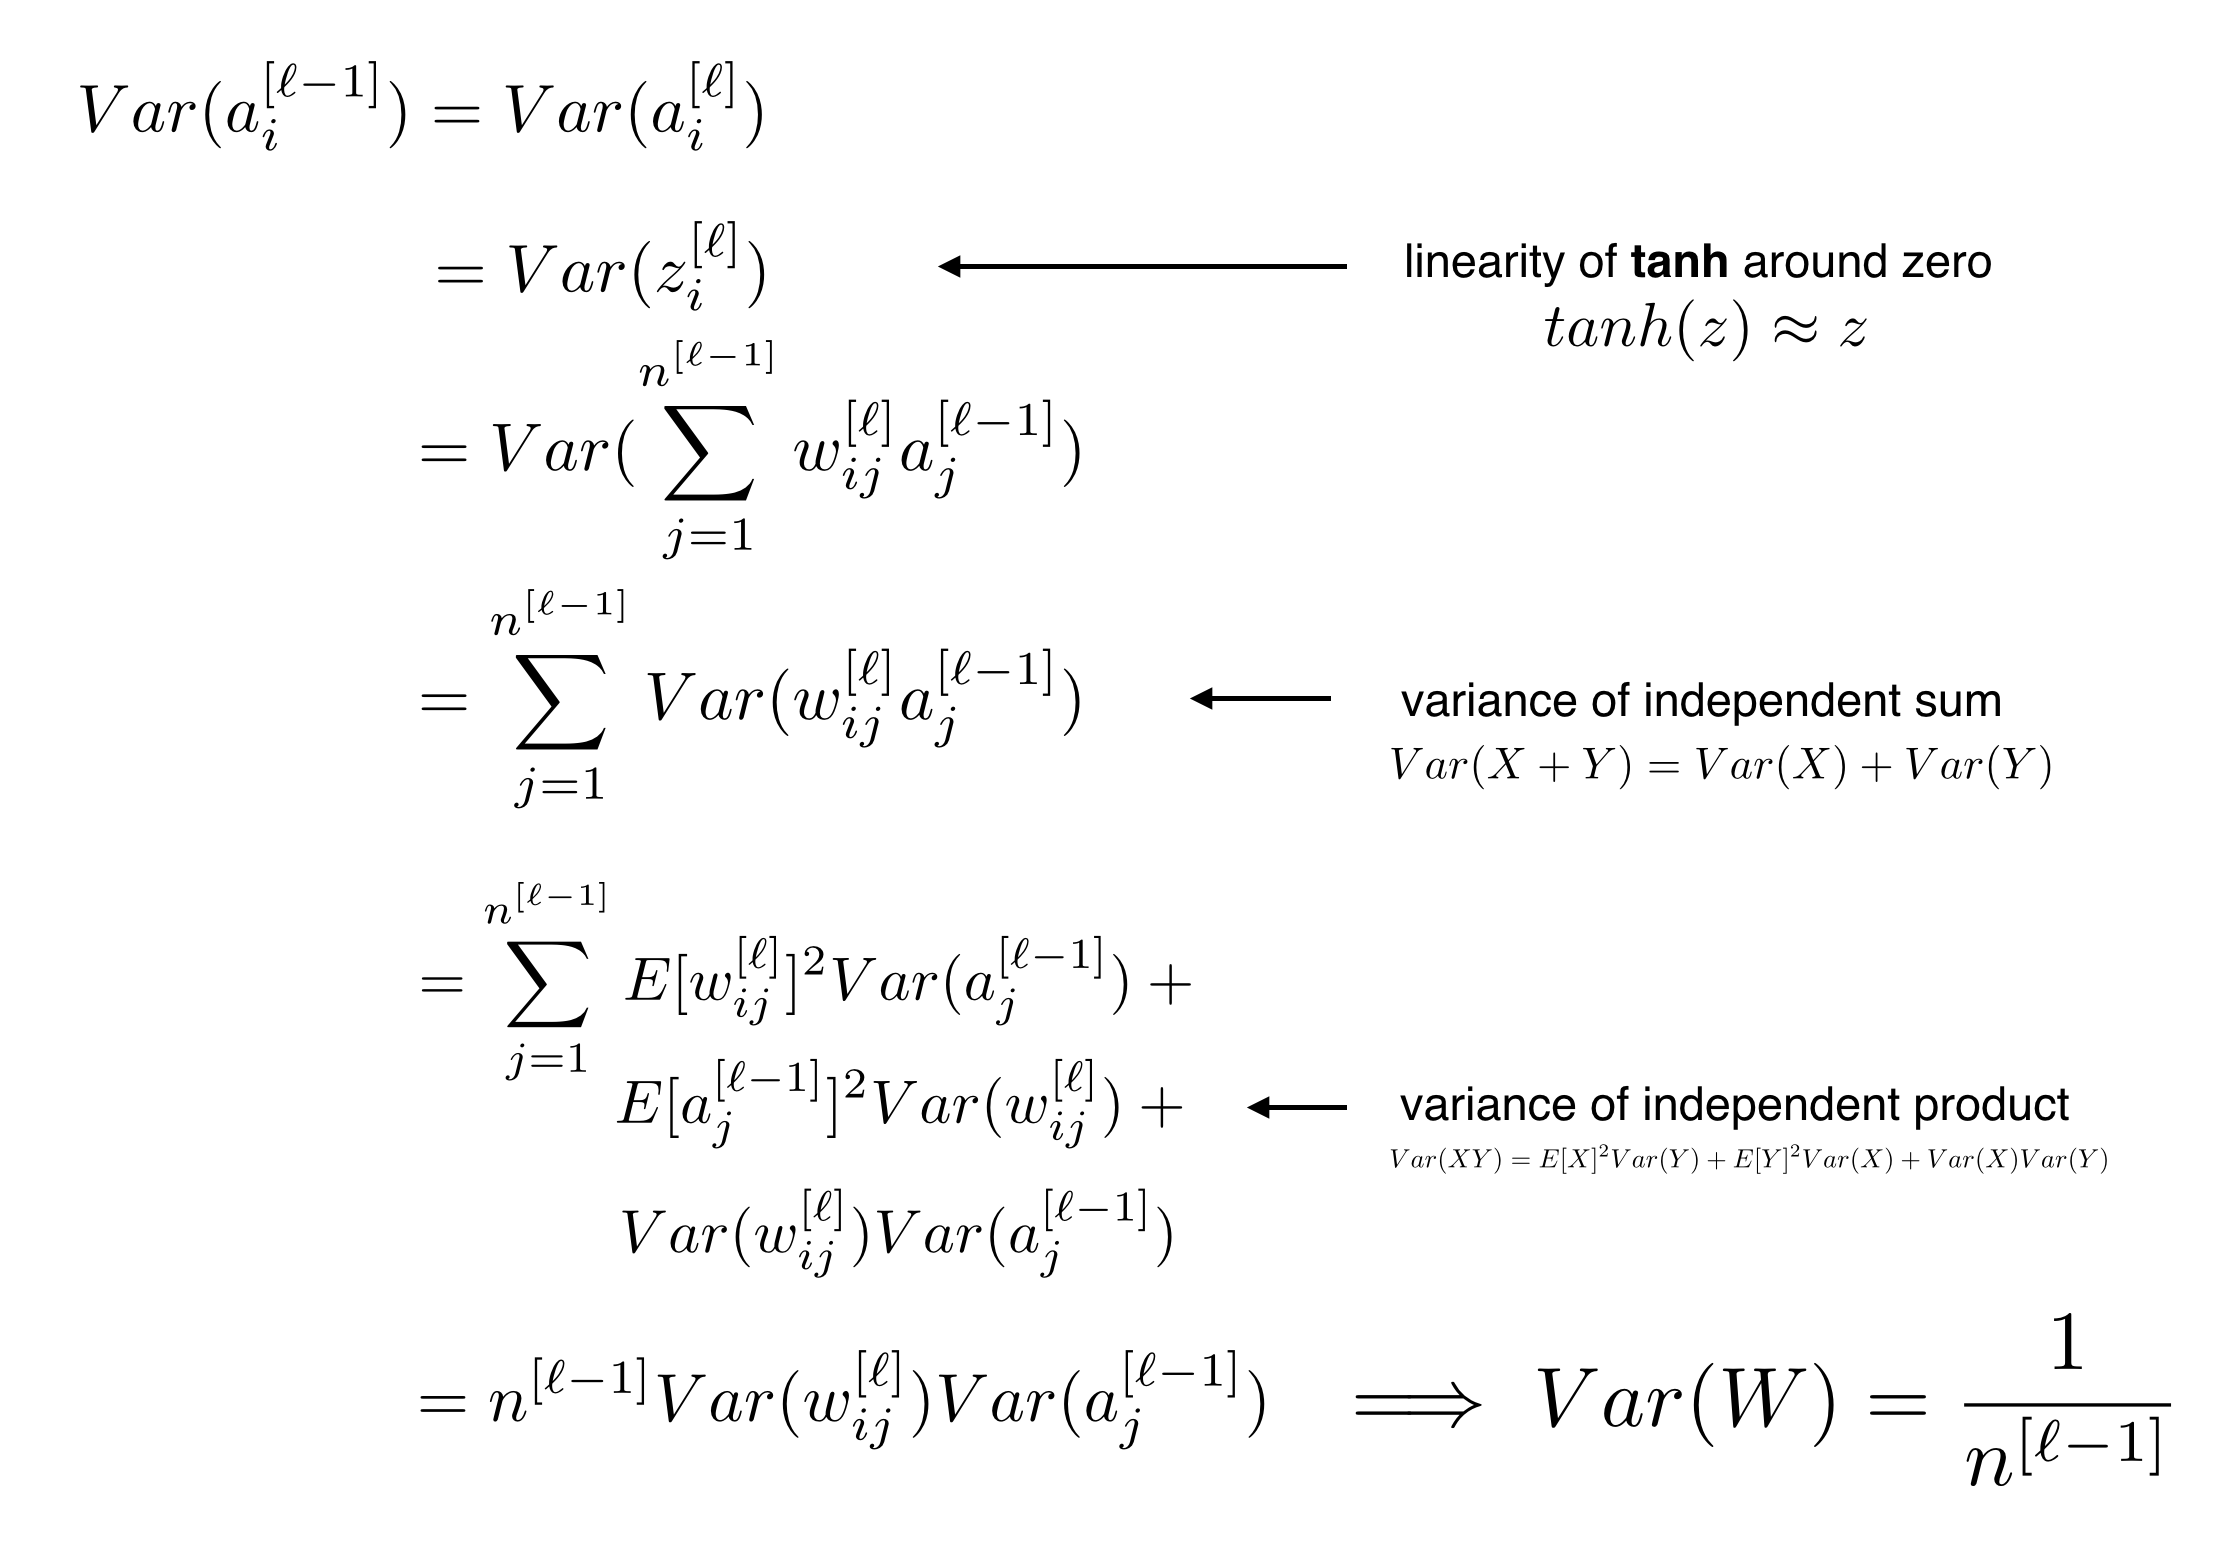
\includegraphics[width=4in]{images/Chapter 10/10.5(3).png}

\end{center}

\end{example}

\begin{example}
How is a$ W_{i}$ calculated when using Xavier initialization?
For a current Layer, let s be the output connections of the layer and e the input connections, then: $ f(W)= \frac{2}{e+s} $

~\\Solution:

In the case of Xavier initialization (also called "Glorot normal" in some software), the parameters are initialized as random draws from a truncated normal distribution with mean 0 and standard deviation

$\sigma = \sqrt{\frac{2}{a+b}}$

where a is the number of input units in the weight tensor, and b is the number of output units in the weight tensor.
\end{example}

\section{Exercises}
\begin{enumerate}
    \item Given $N\vx=[1.0, 0.8, 0.2]$ and $\vy=[1, 1, 0]$, compute the per-example loss for the following functions:
    \begin{enumerate}
        \item Square Error Loss $L_{SE}(N\vx, \vy)$
        \item Cross Entropy Loss $L_{CE}(N\vx, \vy)$
    \end{enumerate}
    \item Given $N\vx=[0.7]$ and $\vy=[1]$, find the Binary Cross Entropy Loss $L_{BCE}(N\vx, \vy)$
    \item How does squared error affect backpropagation? Derive an expression for $\delta^{(D-1)}$ where $L=L_{SE}$
\end{enumerate}

\subsection{Solutions}
\begin{enumerate}
    \item The per-example loss for the functions is:
    \begin{enumerate}
        \item $L_{SE}(N\vx, \vy) = 0.08$
        \item $L_{CE}(N\vx, \vy) = 0.2231435513142097$
    \end{enumerate}
    \item $L_{BCE}(N\vx, \vy) = 0.10536051565782628$
    \item First, let us compute the gradient of the loss function with respect to $N\vx$:
    \begin{align*}
        L_{SE}(N\vx,\vy) &= ||N\vx-\vy||_{2}^{2} \\
        \frac{\partial L_{SE}}{\partial N\vx} &= 2(N\vx-\vy)^\intercal
    \end{align*}
    Then, we can substitute to get
    \begin{align*}
        \delta^{(D-1)} &= \frac{\partial L_{SE}}{\partial N\vx}\cdot\frac{\partial N\vx}{\partial S^{D-1}} \\
        &= 2(N\vx-\vy)^\intercal\cdot\frac{\partial N\vx}{\partial S^{D-1}}
    \end{align*}
\end{enumerate}